
%*******************************************************************************
%*********************************** First Chapter *****************************
%*******************************************************************************
%!TEX root = 0.main.tex

\section{Graph Spherical Convolutions}\label{sec:Graph Spherical Convolutions}
In this chapter we introduce DeepSphere \cite{DeepSphere}, an example of Graph Spherical Convolutional Neural Network that uses a modified version of the HKGL to perform graph convolutions and hierarchical pooling to achieve rotation equivariance, and computational efficiency. Then, in section \ref{sec:Chapter2:pointwise convergence of the Heat Kernel Graph Laplacian on the Sphere} we prove a pointwise convergence result of the full HKGL in the case of the sphere using a regular deterministic sampling scheme. In section \ref{sec:Chapter2:How to build a good graph} we show a way of modifying the original graph of DeepSphere to improve its spectral convergence to $\Delta_{\mathbb S^2}$ while managing to contain the computational costs of graph convolutions. Finally in section \ref{sec:Chapter2:Experimental validation} we study how the graph proposed in section \ref{sec:Chapter2:How to build a good graph} performs in practice when used in a Graph Convolutional Neural Network, comparing its performances to DeepSphere \cite{DeepSphere}.
\subsection{Graph Spherical Convolutional Neural Networks} \label{sec:Chapter1:DeepSphere}
Perraudin et al. \cite{DeepSphere} have proposed a Spherical CNN to process and analyze spherical sky maps, as the Cosmic Radiation map in figure \ref{fig:cosmicradiation}. Sky images are modeled as signals on the vertices of a \textit{sparse} graph $G$ on the vertex set $V$ of the image pixels $(v_i)$ with weights
$$
w_{ij}=\exp \left(-\frac{\norm {v_i-v_j}^2}{4t}\right)
$$
where $t$ is a parameter to optimize. In an earlier work, Belkin et al. \cite{NIPS2006_2989} proved the convergence of eigenvectors of the \textit{full} graph $G$ to the eigenfunctions of the Laplace Beltrami operator $\Delta_\mathbb S^2$, when the data is sampled from a uniform distribution on $\mathbb S^2$ (see Section \ref{sec:Chapter1:theoretical foundations}, theorem \ref{theo:spectral convergence}). For this reason and for the intuition we presented at the beginning of Chapter 2 when introducing the mean equivariance error $\overline E_G$, we expect the construction of Perraudin et al. to work well only for images that were sampled with equi area sampling schemes. On such sampling schemes, since the graph Laplacian eigenvectors well approximate the spherical harmonics, the graph convolution (\ref{eq:graph convolution}) well approximates the true spherical convolution (\ref{eq:convolution}).
\begin{equation}\label{eq:approx}
\mathbf f^T\mathbf v_{i(\ell, m)} \approx \int_{\eta \in \mathbb S^2}f(\eta)Y_\ell^m(\eta)d\mu(\eta)=\hat f(\ell,m)
\end{equation}
The most used sampling scheme by cosmologists and astrophysics is called HEALPix \cite{HEALPix}, and is the one implemented in DeepSphere. HEALPix is an acronym for Hierarchical Equal Area isoLatitude Pixelization of a sphere. This sampling produces a subdivision of the sphere in which each pixel covers the same surface area as every other pixel. It is parametrized by a parameter $N_{side}\in\mathbb N$, and is made of $n=12N_{side}^2$ pixels. The points of this sampling lie on isolatitude rings, making it possible to implement an FFT algorithm for the discrete SHT. The minimal resolution for HEALPix is given by $N_{side}=1$ and is made by 12 pixels. For each increasing value of $N_{side}$ each patch is divided into 4 equal area patches centered around the pixels of the new sampling (figure \ref{fig:healpix sampling}).

In chapter \ref{sec:Chapter4} of this work we'll deepen the relationship between the continuous spherical Fourier transform and the graph Fourier transform in case of non-uniform sampling measures. Perraudin et al. propose an efficient implementation of the graph convolution (\ref{eq:graph convolution}) to be implemented in each layer of their Graph Spherical Convolutional Neural Network. They propose to learn only those filters that are polynomials of degree $q$ of the eigenvalues $\lambda_i$
\begin{equation}\label{eq:deepsphere filter}
\begin{aligned}
k(\lambda) &= \sum_{j=0}^{q} \theta_{j} \lambda^{j}\\ 
\Omega_\mathbf K \mathbf f &= \boldsymbol{V}\left(\sum_{j=0}^{q} \theta_{j} \boldsymbol{\Lambda}^{j}\right) \boldsymbol{V}^{\top} \boldsymbol{f}=\sum_{j=0}^{q} \theta_{j} \boldsymbol{L}^{j} \boldsymbol{f}
\end{aligned}
\end{equation}
Learning the filter $k$ means learning the coefficients $\theta_i$. In this way they solve different problems at once: first, to compute the graph convolution (\ref{eq:graph convolution}) there's no need of computing the expensive eigen decomposition of $\mathbf L$, but they just need to evaluate a polynomial of the sparse matrix $\mathbf L$. Thanks to a suitable parametrization of the polynomial $\sum_{j=0}^{q} \theta_{j} \boldsymbol{L}^{j}$ in term of Chebyshev polynomials, they manage to reduce the computations needed to evaluate such filter to $\mathcal O(|E|)$. Since in a NN this filtering operation has to be computed in every forward and backward pass, this gain in efficiency is dramatically important and led to speedups of different orders of magnitude compared to the architecture of Cohen et al. (see Chapter 2, table \ref{tab:SHREC17_class}). The filtering operation (\ref{eq:deepsphere filter}) can be seen also in the vertex domain as a weighted sum of the $q$-neighborhoods of each vertex. This is due to the fact that $\mathbf L $ has the same sparsity structure of the adjacency matrix of the graph, and thus $(\mathbf L^q)_{ij}$ will be non-zero if and only if the vertices $v_i, v_j$ are connected by a path of length $q$. 

\begin{figure}
	\centering
	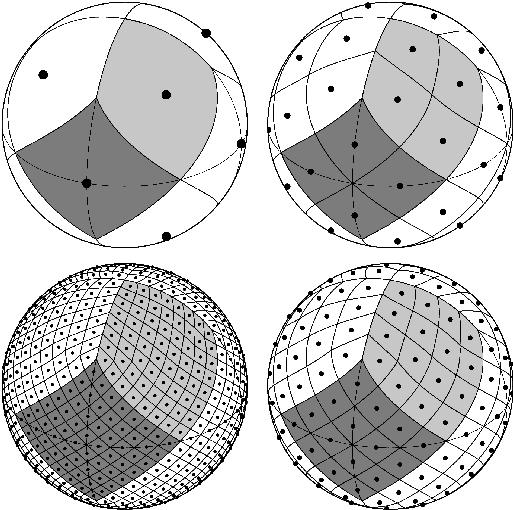
\includegraphics[width=0.5\textwidth]{figs/chapter1/healpix.jpg}
	\caption{\label{fig:healpix sampling}HEALPix sampling for $N_{side}=1,2,3,4$ \cite{HEALPix}}
\end{figure}

 Despite theorem \ref{theo:spectral convergence} \cite{Belkin:2005:TTF:2138147.2138189} states spectral convergence to the continuous Laplace-Beltrami operator for the \textit{full} HKGL, the \textit{sparse} version of the HKGL of Perraudin et al. does not seem to show such convergence. In figure (\ref{fig:Old spectrum1}) we see the correspondence between the subspaces spanned by the graph Fourier modes of the graph Laplacian used by Perraudin et al. and the true spherical harmonics. We can see in figure \ref{fig:Old spectrum} the plot of the graph eigenvalues: we can see that they clearly come in groups of $(2\ell+1)$ eigenvalues corresponding to each $\ell$th degree of the spherical harmonics. We thus call $v_\ell^i$ the $i$th graph eigenmode of degree $\ell$, $|i|\leq\ell$. We compute the normalized Discrete Spherical Harmonic Transform (DSHT) of each $v^i_\ell$ up to the degree $\ell_\text{max}$. The entry $(\ell, \kappa)$ of the matrix represented in the figure corresponds to the percentage of energy of the $\ell$th eigenspace $V_\ell = \text{span}\{v^0_\ell, ..., v^{2\ell+1}_\ell\}$ contained in the $\kappa$th eigenspace of the true spherical harmonics. 
\begin{figure}[h]
	\begin{center}
		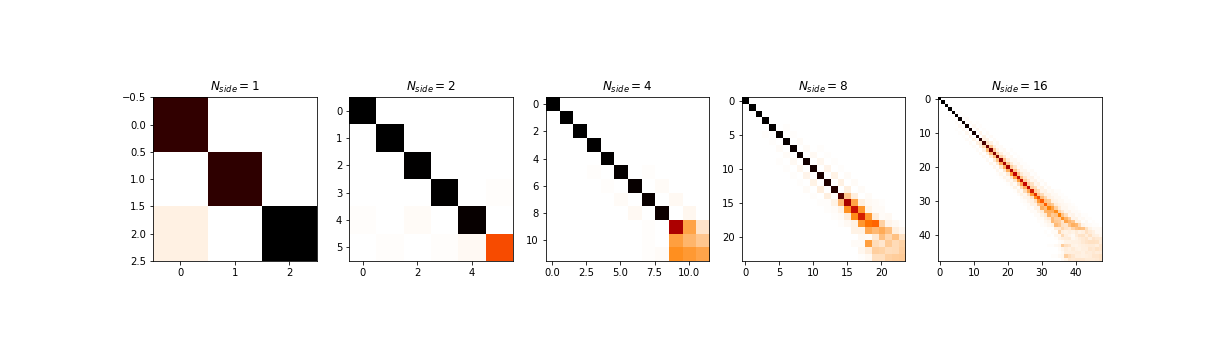
\includegraphics[width=1\linewidth]{../codes/02.HeatKernelGraphLaplacian/HEALPix/06_figures/deepsphere_original.png}
		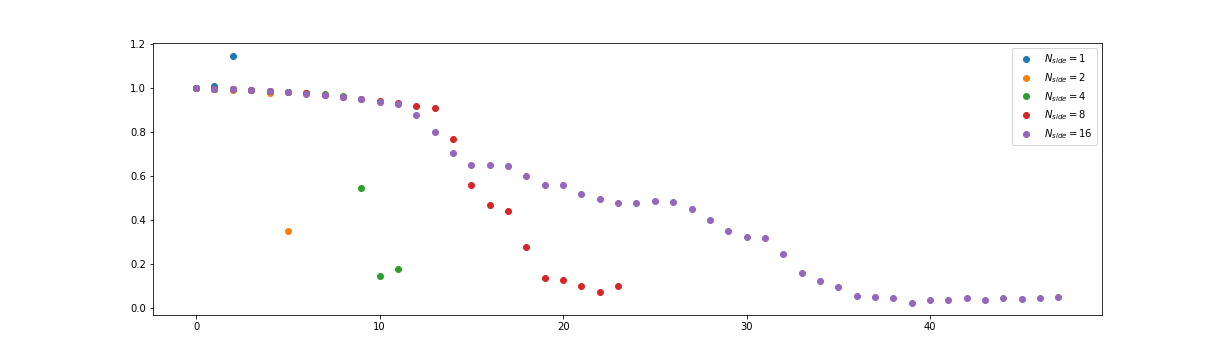
\includegraphics[width=1\linewidth]{../codes/02.HeatKernelGraphLaplacian/HEALPix/06_figures/deepsphere_original_diagonal.png}
		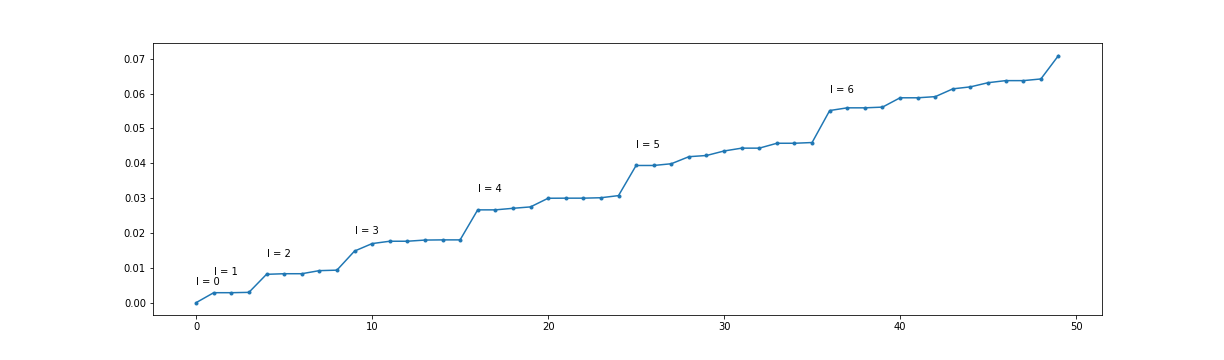
\includegraphics[width=1\linewidth]{../codes/02.HeatKernelGraphLaplacian/HEALPix/05_figs/old_results3.png}
	\end{center}
	\caption{\label{fig:Old spectrum1}Alignment of the graph Laplacian eigenvectors of the DeepSphere graph $W$, the starting point of this work, and its spectrum for $N_{side}=16$.}
\end{figure} 
In a perfect situation, this matrix would be the identity matrix, being all the energy of the $\ell$th graph eigenspace contained in the corresponding one spanned by the true spherical harmonics. It can be seen that the eigenmodes of the graph Laplacian span almost the same subspaces as the spherical harmonics in the low frequencies, but this alignment gets worse at higher frequencies. Furthermore, it can be noticed that even by improving the resolution of the graph, the low frequency eigenspaces do not get better aligned.



\subsection{Pointwise convergence of the Heat Kernel Graph Laplacian on the Sphere}

\label{sec:Chapter2:pointwise convergence of the Heat Kernel Graph Laplacian on the Sphere}
Here we prove a pointwise convergence result of the full graph Laplacian in the case of the sphere on a deterministic sampling that is regular enough. Our proof will be constructed following the ideas presented in the proof of theorem \ref{theo:Belkin pointwise convergence}.
\vspace{0.5cm}
\begin{definition}{}(Heat Kernel Graph Laplacian operator)\\
	\label{def:Heat Kernel Graph Laplacian operator}
	\text{Given a sampling $\{x_i\in\mathcal M\}_{i=0}^{n-1}$ of the manifold we define the \textbf{operator} }$L_n^t$ such that
	$$L_n^tf(y) := \frac{1}{n}\left[ \sum_{i=0}^{n-1} \exp{-\frac{||x_i-y||^2}{4t}}\left(f(y)-f(x_i)\right)\right]$$
\end{definition}
\vspace{0.5cm}
Observe that the Heat Kernel Graph Laplacian operator restricted on the sample points $x_0, ..., x_{n-1}$ acts as the usual Heat Kernel Graph Laplacian matrix $\mathbf L_n^t$ rescaled by a factor of $\frac{1}{n}$:
$$L_n^tf(x_i) = \frac{1}{n} (\mathbf L_n^t\mathbf f)_i$$.
\vspace{0.5cm}
\begin{snugshade*}
\begin{theorem}{from \cite[Belkin et al.]{Belkin:2005:TTF:2138147.2138189}}\\
	\label{theo:Belkin pointwise convergence}
	Let $\mathcal M$ be a $k$-dimensional compact smooth manifold embedded in some euclidean space $\mathbb R^N$, and fix $p\in\mathcal M$. Let the data points $x_1, ... x_n$ be sampled form a uniform distribution on the manifold $\mathcal M$. Set $t_n=n^{-\frac{1}{k+2+\alpha}}$, for any $\alpha>0$ and let $f\in\mathcal C_\infty(\mathcal M)$. Then:
	
	$$\forall \epsilon>0\quad \mathbb{P}\left[\left|\frac{1}{t}\frac{1}{(4 \pi t)^{k/2}}L_{n}^{t_n} f(p)-  \frac{1}{\text{vol}(\mathcal M)}L^{t_n} f(p)\right|>\epsilon\right] \xrightarrow{n\to\infty} 0$$
\end{theorem}
\end{snugshade*}
\vspace{0.5cm}
This theorem states a convergence in probability of $L_n^t$ to $L^t$, that is far from being as strong as spectral convergence of theorem \ref{theo:spectral convergence}. However, we want to show that a similar result still holds in the specific case of the manifold $\mathcal M$ being the 2-Sphere $\mathbb S^2$ and where the points $x_1, ..., x_n$ are not sampled from a random distribution on $\mathbb S^2$, but are defined by the HEALPix sampling. To understand the differences between theorem \ref{theo:Belkin pointwise convergence} and theorem \ref{theo:pointwise convergence in the healpix case} it is useful to first review the proof of theorem \ref{theo:Belkin pointwise convergence}. For this proof we'll need to use the Hoeffding's inequality that we recall here under:

(\textit{Hoeffding's inequality})\\
Let \(X_{1}, \ldots, X_{n}\) be independent identically distributed random variables, such that
\(\left|X_{i}\right| \leqslant K .\) Then
\begin{equation}\label{eq:Hoeffding}
\mathbb P\left\{\left|\frac{\sum_{i} X_{i}}{n}-\mathbb{E} X_{i}\right|>\epsilon\right\}<2 \exp \left(-\frac{\epsilon^{2} n}{2 K^{2}}\right)
\end{equation}

\begin{proof}[Proof of Theorem \ref{theo:Belkin pointwise convergence}]
 The first step is to observe that for any fixed $t>0$, any fixed function $f$ and a fixed point $y\in\mathbb S^2$,  the Heat Kernel Graph Laplacian $L_n^t$ is an unbiased estimator for the Functional Approximation of the Laplace-Beltrami $L^t$. In other words, $L_n^tf(y)$ is the empirical average of $n$ i.i.d. random variables $X_i= e^{-\frac{||x_i-y||^2}{4t}}\left(f(y)-f(x_i)\right)$ with expected value corresponding to $L^tf(y)$. Thus,
\begin{equation}
\label{eq:expected value of heat kernel grah laplacian}
	\mathbb E L_n^tf(y) = 	\mathbb E \frac{1}{n}X_i = \mathbb E X_i = L^tf(y),
\end{equation}
and by the strong law of large numbers we have that
\begin{equation}
\label{eq:convergence in probability}
\lim_{n\to\infty}L_n^tf(y) = L^t(y).
\end{equation}
The core of the work of Belkin et al. is the proof, that we will not discuss, of the following proposition.

\begin{prop} Under the same hypothesis of theorem \ref{theo:Belkin pointwise convergence}, we have the following pointwise convergence
	$$\frac{1}{t}\frac{1}{(4\pi t)^{k/2}} L^tf(p) \xrightarrow{t\to 0 } \frac{1}{\text{vol}(\mathcal M)}\triangle_{\mathcal M}f(p).$$
	\label{prop:3}
\end{prop}
Thanks to Proposition \ref{prop:3} and equation (\ref{eq:convergence in probability}), a straightforward application of Hoeffding's inequality with $K=\frac{1}{t}\frac{1}{(4\pi t)^{k/2}}$ together with equation  (\ref{eq:expected value of heat kernel grah laplacian}) leads to

\begin{equation}
	\label{eq:hoeffding applied}
	\mathbb{P}\left[\frac{1}{t(4 \pi t)^{k / 2}}\left|L_{n}^{t} f(y)- L^{t} f(y)\right|>\epsilon\right] \leq 2 e^{-1 / 2 \epsilon^{2} n t(4 \pi t)^{k / 2}}
\end{equation}

We want the right hand side of equation (\ref{eq:hoeffding applied}) to go to $0$ for $n\to\infty, t\to0$ at the same time. For this to happen, we need to find a sequence $(t_n)$ such that 
$$\begin{cases}
t_n\xrightarrow{n\to\infty}0\\
2 e^{-1 / 2 \epsilon^{2} n t_n(4 \pi t_n)^{k / 2}}\xrightarrow{n\to\infty}0\\
\end{cases}$$

By fixing $t_n=n^{-\frac{1}{k+2+\alpha}}$, for any $\alpha>0$, it is easy to check that \\$-1 / 2 \epsilon^{2} n t_n(4 \pi t_n)^{k / 2}\xrightarrow{n\to\infty}+\infty$, thus concluding the proof.

\end{proof}

Now we can observe that in order to adapt this proof to the case of the sphere with an equi area sampling scheme we need to modify two key things. First, due to the deterministic nature of the sampling scheme, we need to prove that for any fixed $t>0$, any fixed function $f$ and any point $y\in\mathbb S^2$ 
\begin{equation}\label{eq:limit}
	\left|L_n^tf(y)-L^tf(y)\right|\xrightarrow{n\to \infty} 0,
\end{equation}
without relying on the strong law of large numbers. Once proven such result, we need to prove that

$$\left|\frac{1}{4\pi t^2}\left(L_n^tf(x) - L^tf(x)\right)\right|\xrightarrow[n\to \infty]{t\to 0}0$$

We need now to define some geometrical quantities that we'll need. Given a sampling $x_0, ..., x_{n-1}$ define $\sigma_i$ to be the patch of the surface of the sphere corresponding to the $i$th point of the sampling, define $A_i$ to be its corresponding area and $d_i$ to be the radius of the smallest ball in $\mathbb R^3$ containing the i-th patch (see Figure \ref{fig:Geometric characteristics of a patch}). Define $d^{(n)} := \max_{i=0, ..., n}d_i$ and $A^{(n)}=\max_{i=0, ..., n}A_i$.\\
Once proven the limit (\ref{eq:limit}), Proposition \ref{prop:3} leads to our main result:
\vspace{1cm}
\begin{snugshade*}
	\begin{theorem}
		For a sampling $\mathcal P = \{x_i\in\mathbb S^2\}_{i=0}^{n-1}$ of the sphere that is equi area and such that $d^{(n)})\leq \frac{C}{\sqrt{n}}$, for all $f: \mathbb S^2 \rightarrow \mathbb R$ Lipschitz with respect to the euclidean distance in $\mathbb R^3$, for all $y\in\mathbb S^2$, there exists a sequence $t_n = n^\beta$ such that the rescaled Heat Kernel Graph Laplacian operator $\frac{|\mathbb S^2|}{4\pi t_n}L^t_n$ converges pointwise to the Laplace Beltrami operator on the sphere $\triangle_{\mathbb S^2}$  for $n\to\infty$:
		$$ \lim_{n\to\infty}\frac{|\mathbb S^2|}{4\pi t_n} L_n^{t_n}f(y) =  \triangle_{\mathbb S^2}f(y).$$
		\label{theo:pointwise convergence in the healpix case}
	\end{theorem}
\end{snugshade*}

\vspace{1cm}
\begin{minipage}{.4\textwidth}
	\centering
	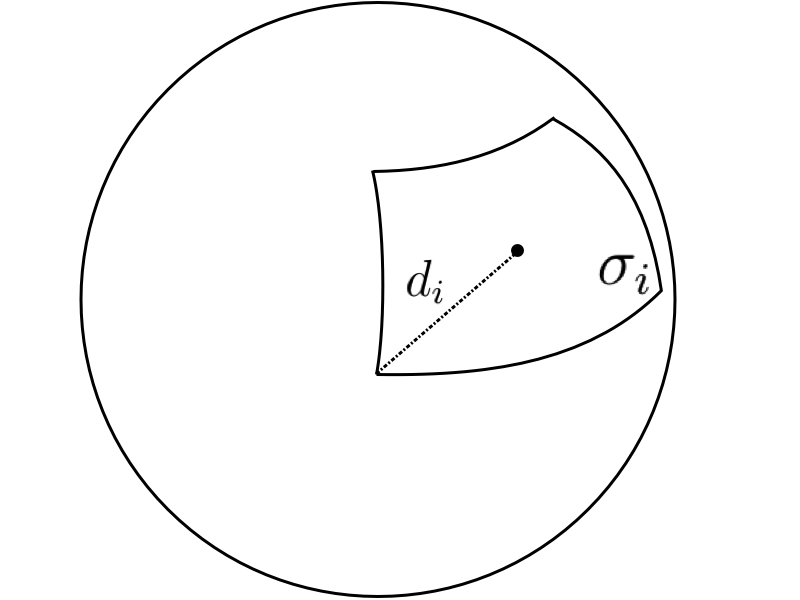
\includegraphics[width=0.8\linewidth]{figs/chapter1/d_iA_i.jpg}
	\captionof{figure}{\label{fig:Geometric characteristics of a patch}Geometric characteristics of the $i$th patch}
\end{minipage}%
\hfill
\begin{minipage}{.5\textwidth}
	\centering
	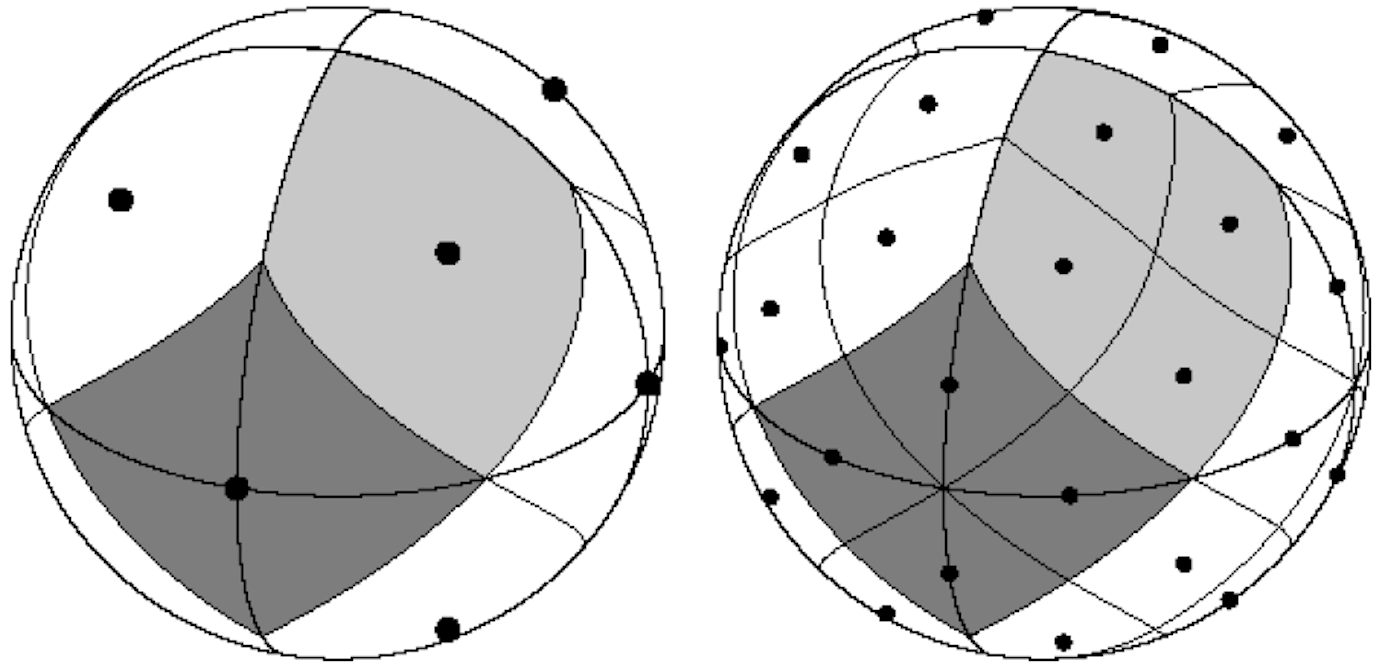
\includegraphics[width=\linewidth]{figs/chapter1/Heal_Base.png}
	\captionof{figure}{\label{fig:HEALPix equal areas patches}HEALPix equal areas patches for $N_{side}=1$, $N_{side}=2$}
	\vspace{0.5cm}
\end{minipage}

\subsubsection{Proof of the pointwise convergence of the Heat Kernel Graph Laplacian on the Sphere for an equi area sampling scheme}

Our first goal is to prove the following Proposition: 
\vspace{0.5cm}
\begin{prop}\label{prop:1}
	For an equal area sampling $\{x_i\in\mathbb S^2\}_{i=0}^{n-1}: A_i=A_j \forall i,j$ of the sphere it is true that for all $f: \mathbb S^2 \rightarrow \mathbb R$ Lipschitz with respect to the euclidean distance $||\cdot||$ with Lipschitz constant $\mathcal L_f$ 
	$$
	\left| \int_{\mathbb S^2}f({ x})\text{d}{\mu(x)} - \frac{1}{n}\sum_i f( x_i)\right|\leq \mathcal L_fd^{(n)}.
	$$
	Furthermore, for all $y\in\mathbb S^2$ the Heat Kernel Graph Laplacian operator $L^t_n$ converges pointwise to the functional approximation of the Laplace Beltrami operator $L^t$
	$$ L_n^tf(y)\xrightarrow{n\to\infty} L^tf(y).$$
\end{prop} 
\vspace{0.5cm}


\begin{proof}
	Let us assume that the function $f:\mathbb R^3\rightarrow \mathbb R$ is Lipschitz with Lipschitz constant $\mathcal L_f$, we have 
	
	$$\left| \int_{\sigma_{i}}f({ x})\text{d}{\mu(x)} - \frac{1}{n}f( x_i)\right| \leq \mathcal L_fd^{(n)}\frac{1}{n} $$

	So, by triangular inequality and by summing all the contributions of all the $n$ patches
	$$\left| \int_{\mathbb S^2}f({ x})\text{d}{\mu(x)} - \frac{1}{n}\sum_i f( x_i)\right| \leq \sum_i \left| \int_{\sigma_{i}}f({ x})\text{d}{\mu(x)} - \frac{1}{n}f( x_i)\right|\leq n  \mathcal L_fd^{(n)}\frac{1}{n} = \mathcal L_fd^{(n)}$$	
	Thanks to this result, we have the following two pointwise convergences
	
	$$\forall f \text{ Lipschiz,}\quad \forall y\in\mathbb S^2,  \quad\quad \frac{1}{n}\sum_i e^{-\frac{||x_i-y||^2}{4t}}\rightarrow \int e^{-\frac{||x-y||^2}{4t}}d\mu(x)$$
	$$\forall f \text{ Lipschiz,}\quad \forall y\in\mathbb S^2,  \quad\quad \frac{1}{n}\sum_i e^{-\frac{||x_i-y||^2}{4t}}f(x_i)\rightarrow \int e^{-\frac{||x-y||^2}{4t}}f(x)d\mu(x)$$
	
	Definitions \ref{def:Heat Kernel Graph Laplacian operator} and \ref{def:Functional approximation to the Laplace-Beltrami operator} end the proof.
\end{proof}
\vspace{0.5cm}

Now, we just proved that \textit{keeping t fixed} $L_n^tf(x)\rightarrow L^tf(x)$. Now our goal is to prove that:

\vspace{0.5cm}
\begin{prop}\label{prop:2}
	Given a sampling regular enough i.e., for which we assume $A_i=A_j \ \forall i,j\text{ and }d^{(n)}\leq \frac{C}{\sqrt{n}}$, for a fixed $t>0$, a fixed Lipschitz function $f$ and a fixed point $y\in\mathbb S^2$ there exists a sequence $t_n = n^\beta, \beta<0$ such that 
$$
\forall f \text{ Lipschitz, } \forall x\in\mathbb S^2 \quad \left|\frac{1}{4\pi t_n^2}\left(L_n^{t_n}f(x) - L^{t_n}f(x)\right)\right|\xrightarrow{n\to \infty}0.
$$
\end{prop}
\vspace{0.5cm}

The main result of this section, theorem  \ref{theo:pointwise convergence in the healpix case}, is then an immediate consequence of Proposition \ref{prop:2} and Proposition \ref{prop:3}.


\begin{proof}[Proof of Proposition \ref{prop:2}]
	
	We define for simplicity of notation
	\begin{align*}
		\phi^t(x;y) &:= e^{-\frac{||x-y||^2}{4t}}\left(f(y)-f(x)\right)\\
		K^t(x,y) &:=  e^{-\frac{||x-y||^2}{4t}}
	\end{align*}
	We start by writing the following chain of inequalities
	\begin{align*}
		||L_n^tf-L^tf||_\infty &= \max _{y\in \mathbb S^2} \left|L_n^tf(y)-L^tf(y)\right|\\
		&= \max _{y\in \mathbb S^2} \left| \frac{1}{n} \sum_{i=1}^n \phi^t(x_i; y)- \int_{\mathbb S^2} \phi^t(x;y)d\mu(x) \right|\\
		&\leq \max _{y\in \mathbb S^2}  \sum_{i=1}^n   \left| \frac{1}{n}  \phi^t(x_i; y)- \int_{\sigma_i} \phi^t(x;y)d\mu(x) \right|\\
		&\leq  \max _{y\in \mathbb S^2} \left[\mathcal L_{\phi^t_y}d^{(n)} \right]\\
	\end{align*}
	where $\mathcal L_{\phi^t_y}$ is the Lipschitz constant of $x \rightarrow \phi^t(x, y)$ and where we used for the last inequality Proposition \ref{prop:1}. If we assume $d^{(n)}\leq \frac{C}{\sqrt{n}}$ we have that
	
	$$||L_n^tf-L^tf||_\infty  \leq  \max _{y\in \mathbb S^2} \left[ \mathcal L_{\phi^t_y} \frac{C}{\sqrt{n}} \right]$$
	
	Let's now find the explicit dependence $t\rightarrow \mathcal L_{\phi^t_y}$
	\begin{align*}
		\mathcal L_{\phi^t_y} &= ||\partial_x\phi^t(\cdot;y)||_\infty\\&
		= ||\partial_x\left(K^t(\cdot;y)f\right)||_\infty\\&
		= ||\partial_x K^t(\cdot;y)f + K^t(\cdot;y)\partial_x f||_\infty\\&
		\leq ||\partial_x K^t(\cdot;y)f||_\infty + ||K^t(\cdot;y)\partial_x f||_\infty\\&
		\leq  ||\partial_x K^t(\cdot;y)||_\infty||f||_\infty + ||K^t(\cdot;y)||_\infty||\partial_x f||_\infty\\&
		= ||\partial_x K^t(\cdot;y)||_\infty||f||_\infty + ||\partial_x f||_\infty\\&
		= \mathcal L_{K^t_y} ||f||_\infty + ||\partial_xf||_\infty\\&
		= \mathcal L_{K^t_y} ||f||_\infty + \mathcal L_f
	\end{align*}
	where $\mathcal L_{K^t_y}$ is the Lipschitz constant of $x\rightarrow K^t(x;y)$. We can observe that such constant does not depend on $y$:
	
	$\mathcal L_{K^t_y} = \norm{\partial_x e^{-\frac{x^2}{4t}}}_\infty = \norm{\frac{x}{2t}e^{-\frac{x^2}{4t}}}_\infty = \left. \frac{x}{2t}e^{-\frac{x^2}{4t}}\right|_{x=\sqrt{2t}}=(2et)^{-\frac{1}{2}}\propto t ^ {-\frac{1}{2}}$
	
	So we can continue
	\begin{align*}
		\max _{y\in \mathbb S^2} \left[  \mathcal L_{\phi^t_y} \frac{C}{\sqrt{n}} \right]
		&\leq  \frac{C}{\sqrt{n}} \left( (2et)^{-\frac{1}{2}} \norm{f}_\infty + \mathcal L_f \right)\\
		&\leq \frac{C\norm{f}_\infty}{\sqrt{n}(2et)^\frac{1}{2}} +   \frac{C}{\sqrt{n}}\mathcal L_f\\
	\end{align*}
	So we have that, rescaling by a factor $\frac{1}{4\pi t^2}$
	\begin{align*}
		\norm{\frac{1}{4\pi t^2}\left(L_n^tf-L^tf\right)}_\infty&\leq \frac{1}{4\pi t^2}\norm{\left(L_n^tf-L^tf\right)}_\infty \\
		&\leq \frac{C}{4\pi}\left[\frac{\norm{f}_\infty}{\sqrt{2e}}\frac{1}{\sqrt{n}t^\frac{5}{2}} + \frac{\mathcal L_f}{\sqrt{n}t^2}\right]
	\end{align*}

	
	we want $\begin{cases}
	t \rightarrow 0\\
	n \rightarrow \infty\\
	\sqrt{n}t^\frac{5}{2} \rightarrow \infty\\
	\sqrt{n}t^2 \rightarrow \infty
	\end{cases}$ in order for $ \frac{C}{4\pi}\left[\frac{\norm{f}_\infty}{\sqrt{2e}}\frac{1}{\sqrt{n}t^\frac{5}{2}} + \frac{\mathcal L_f}{\sqrt{n}t^2}\right] \xrightarrow[t\to 0 ]{n\to\infty}0$
	
	This is true if $\begin{cases}
	t(n) = n^\beta, &\beta\in(-\frac{1}{5}, 0) \\
	t(n) = n^\beta, &\beta\in(-\frac{1}{4}, 0)
	\end{cases} \implies t(n) = n^\beta, \quad \beta\in(-\frac{1}{5}, 0)$
	
	Indeed 
	
	$\sqrt{n}t^\frac{5}{2}=n^{5/2\beta+1/2}\xrightarrow{n \to \infty} \infty$ since $\frac{5}{2}\beta+1/2>0 \iff \beta>-\frac{1}{5}$
	
	$\sqrt{n}t^2=n^{2\beta+1/2}\xrightarrow {N \to \infty} \infty$ since $2\beta+1/2>0 \iff \beta>-\frac{1}{4}$
	
	So, for $t=n^\beta$ with $\beta\in(-\frac{1}{5}, 0)$ we have that 
	
	$$\begin{cases}
	(t_n)\xrightarrow{n\to\infty}0\\
	\norm{\frac{1}{4\pi t_n^2}L_n^{t_n}f-\frac{1}{4\pi t_n^2}L^{t_n}f}_\infty  \xrightarrow{n\to\infty}0
	\end{cases}$$
	
\end{proof}

The proof of theorem \ref{theo:pointwise convergence in the healpix case} is now trivial:
\begin{proof}[Proof of Theorem \ref{theo:pointwise convergence in the healpix case}]
	Thanks to Proposition \ref{prop:2} and Proposition \ref{prop:3}	we conclude that $\forall y\in\mathbb S^2 $
	$$\lim_{n\to\infty}\frac{1}{4\pi t_n^2} L_n^{t_n}f(y) =  \lim_{n\to\infty}\frac{1}{4\pi t_n^2} L^{t_n}f(y) = \frac{1}{|\mathbb S^2|}\triangle_{\mathbb S^2}f(y) $$
\end{proof}

The proof of this result is instructive since it shows that we need to impose some regularity conditions on the sampling. If the sampling is equal area as HEALPix, meaning that all the patches $\sigma_i$ have the same area (i.e., HEALPix, see figure \ref{fig:HEALPix equal areas patches}), then we need to impose that $ d^{(n)}\leq \frac{1}{\sqrt{n}}$. If the sampling is not equal area, meaning that in general $A_i\neq A_j$, it can be shown that we need a slightly more complex condition: $\max_{i=0,...,n-1}d_iA_i\leq Cn^{-\frac{3}{2}}$.\\
In the work of Belkin et al. \cite{Belkin:2005:TTF:2138147.2138189} the sampling is drawn form a uniform random distribution on the sphere, and their proof heavily relies on the uniformity properties of the distribution from which the sampling is drawn. In our case the sampling is deterministic, and the fact that for a sphere there doesn't exist a regular sampling with more than 12 points (the vertices of a icosahedron) is indeed a problem that we need to overcome by imposing the regularity conditions above. 


To conclude, we can see that the result obtained has the same form than the result obtained in \cite{Belkin:2005:TTF:2138147.2138189}. Given the kernel density $t(n)=n^\beta$, if Belkin et al. proved convergence in the random case for $\beta \in (-\frac{1}{4}, 0)$, we proved convergence in the HEALPix case for $\beta \in (-\frac{1}{5}, 0)$. This kind of result can be interpreted in the following way. In order to have this pointwise convergence, we need to reduce the kernel width but \textit{not so fast} compared to the resolution of the graph. In other words, the kernel width has to be reduced but is somewhat limited by the resolution of the graph. In the next section we'll see how to set in practice a good kernel width $t$ given a graph resolution $n$.
\begin{remark}
	Pointwise convergence is just a necessary condition for spectral convergence.  Theorem \ref{theo:pointwise convergence in the healpix case} does not imply convergence of eigenvalues and eigenvectors.
\end{remark}

\subsection{How to build a good graph to approximate spherical convolutions}
\label{sec:Chapter2:How to build a good graph}
The current state of the art of rotation equivariant Graph CNN is DeepSphere \cite{DeepSphere}. However, if we measure the alignment of the eigenspaces spanned by the eigenvectors of the graph Laplacian used in \cite{DeepSphere} and the ones spanned by the spherical harmonics we see that it does not get better as $N_{side}$ increases (figure \ref{fig:deepsphere results}). We'll see that the main cause of this bad behavior of the eigenspaces is the fixed number of neighbors used in \cite{DeepSphere} for the construction of the graph. In this subsection we'll see that to obtain the desired spectral convergence it is necessary to increase the number of neighbors as we decrease the kernel width $t$. We'll follow in practice what we did in proving theorem \ref{theo:pointwise convergence in the healpix case}: first we'll build a \textit{full graph}, and let the number of pixels $n$ increases while keeping the kernel width $t$ fixed. After having discussed the results, we'll try to find a possible sequence $(t_n)$ in order to obtain the expected spectral convergence. Only in the end we'll find a way to make the graph sparse to limit the computational costs of graph convolutions but keeping the eigen decomposition of the graph Laplacian as close to the spherical harmonics as possible.
\begin{figure}[h!]
	\centering
	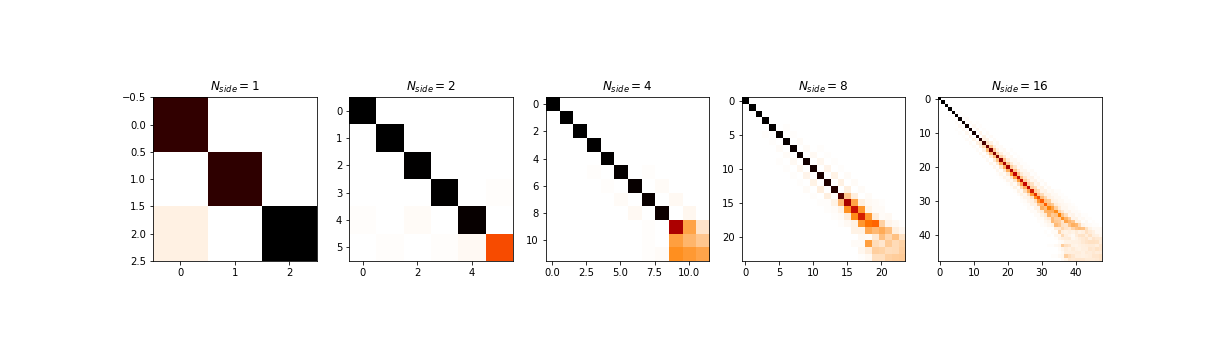
\includegraphics[width=\textwidth]{../codes/02.HeatKernelGraphLaplacian/HEALPix/06_figures/deepsphere_original.png}
		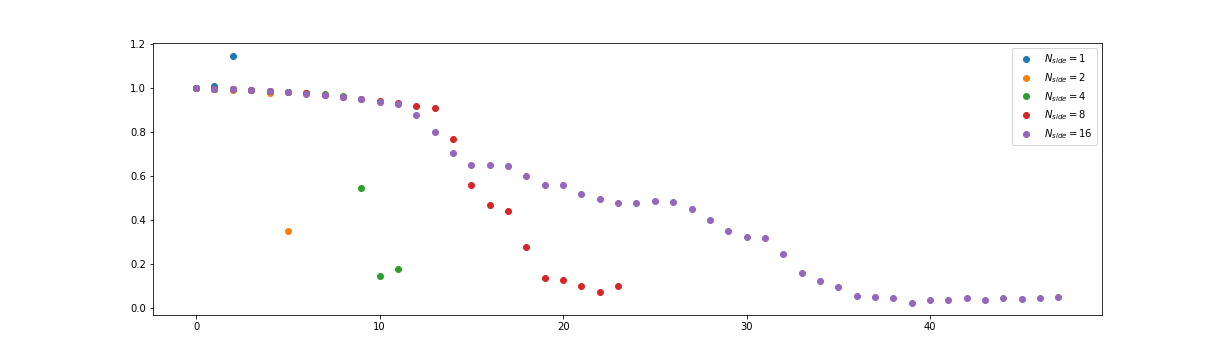
\includegraphics[width=\textwidth]{../codes/02.HeatKernelGraphLaplacian/HEALPix/06_figures/deepsphere_original_diagonal.png}	
		\caption{\label{fig:deepsphere results}Correspondence between the subspaces spanned by the graph Fourier modes and the spherical harmonics of the graph Laplacian of DeepSphere.}
\end{figure}

\subsubsection{Full graph, $n\to\infty$}\label{sec:Chapter1: n to infty}
Here we analyze what happens to the power density spectrum of the \textit{full} Heat Kernel Graph Laplacian as we make $n$ go to infinity while keeping $t$ fixed. Since in the previous section we proved that (Proposition \ref{prop:3}) for a sampling regular enough and a fixed $t$, a fixed function $f$, a fixed point $y$
$$L_n^tf(y)\xrightarrow{n\to\infty}L^tf(y)$$
Since HEALPix is a very regular sampling of the sphere, we expect to observe (even if we didn't prove it) the corresponding spectral convergence proved in theorem \ref{theo:spectral convergence}. The results obtained are in figure \ref{fig:n to infinity1}, \ref{fig:n to infinity3}.

\begin{figure}[h!]
	\centering
	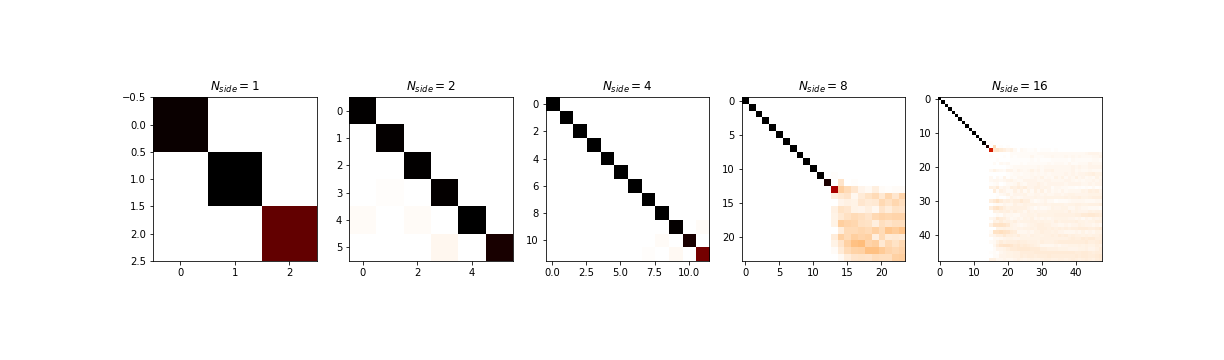
\includegraphics[width=\textwidth]{../codes/02.HeatKernelGraphLaplacian/HEALPix/06_figures/n.png}
	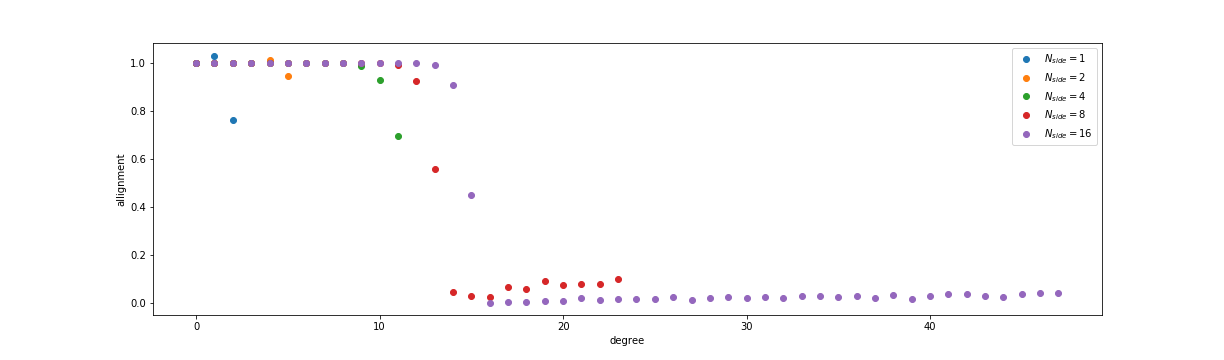
\includegraphics[width=\textwidth]{../codes/02.HeatKernelGraphLaplacian/HEALPix/06_figures/n_diagonal.png}	
	\caption{\label{fig:n to infinity1}Alignment of the eigenvectors of the HKGL with a fixed kernel width $t$}
	
\end{figure}
\begin{figure}[h!]
	\centering
	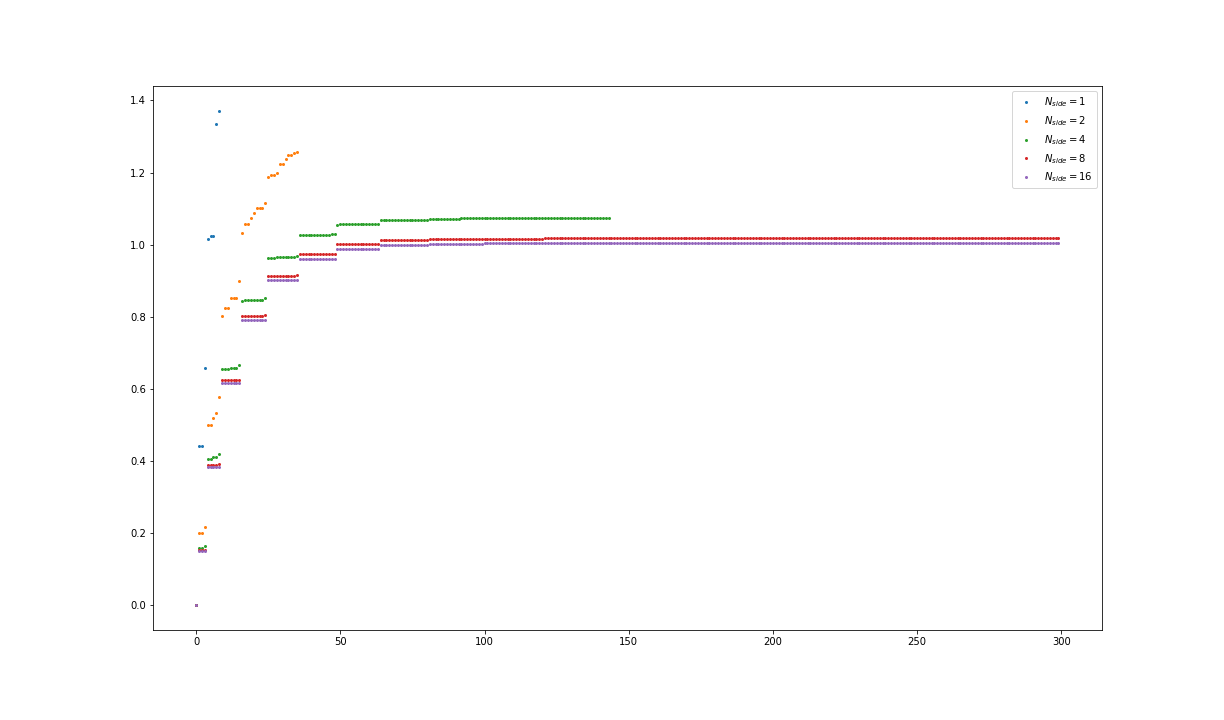
\includegraphics[width=0.49\textwidth]{../codes/02.HeatKernelGraphLaplacian/HEALPix/06_figures/n_eigenvalues.png}
		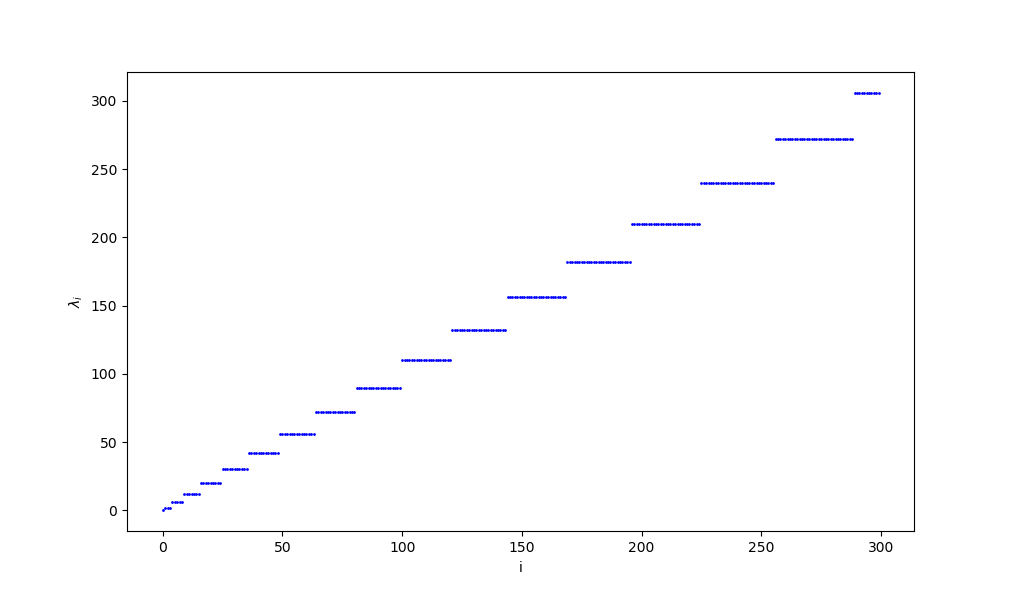
\includegraphics[width=0.49\textwidth]{figs/chapter1/trueeigenvalues.png}	
	\caption{\label{fig:n to infinity3}Left: spectrum of the HKGL with a fixed kernel width $t$. Right: true spectrum of $\Delta_{\mathbb S^2}$}
\end{figure}

In figure \ref{fig:n to infinity1} we see two things: first that there's a frequency threshold beyond which the Graph Laplacian is completely blind, approximately located at the 15th degree, and second that before this frequency threshold, we actually see the convergence expected: the alignment gets better as $n$ gets bigger.

\begin{figure}[h!]
	\centering
	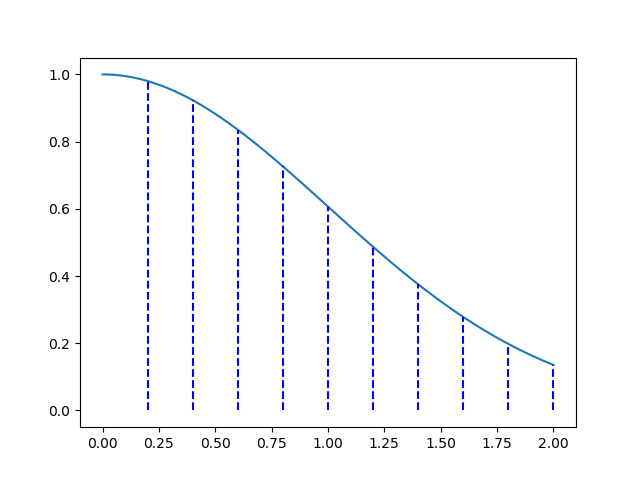
\includegraphics[width=0.45\textwidth]{figs/chapter1/frequency_threshold1.png}	\hfill
	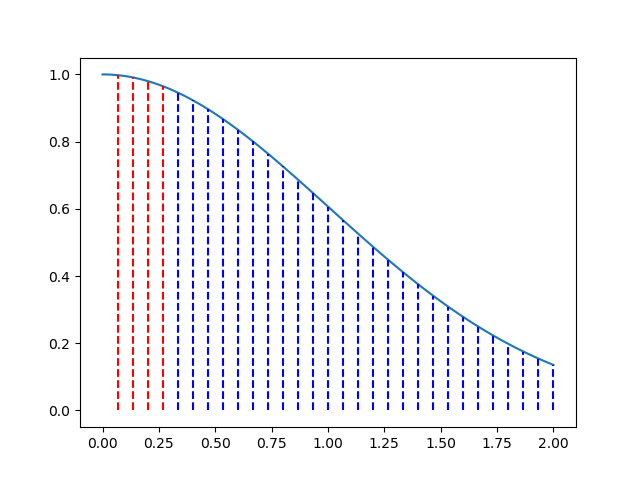
\includegraphics[width=0.45\textwidth]{figs/chapter1/frequency_threshold2.png}	
	\caption{\label{fig:n to infinity4}Frequency threshold explained.}
\end{figure}


 To explain this we refer to figure \ref{fig:n to infinity4} where we show a simplified situation where we are sampling the interval $[0, 2]$ and we plot the Gaussian kernel centered around the first pixel of the sampling corresponding to the origin. On the leftmost image the pixels are correctly spaced with respect to the kernel width, in the sense that the values of the kernel evaluated on the pixels are well far apart from each other. This makes the graph able to "see" all the pixels differently, and thus all the frequencies with wavelength around the order of magnitude of the average pixel distance will be captured by the graph. On the rightmost image in figure \ref{fig:n to infinity4} there are too many pixels with respect to the kernel width: the values of the kernel evaluated on the pixels close to the origin, because of the slope of the kernel being almost zero are too close to each other (in red); because of this any variation of a signal on the red pixels would be almost invisible to the graph Laplacian. With this fixed kernel width $t$, no matter how much we sample the interval $[0,2]$, any frequency with wavelength shorter than the radius $r\approx0.25$ becomes invisible to the graph Laplacian.\\
 This phenomenon can be seen also in the spectrum represented in figure \ref{fig:n to infinity3} where we plot the eigenvalues of the matrix $\mathbf L_n^t$: as $N_{side}$ gets bigger the eigenvalues get more and more grouped in the usual groups of the same multiplicity of the corresponding spherical harmonics; however, there's a frequency (corresponding approximately to the degree $\ell=15$) from which all the eigenspaces tend to merge into one, corresponding to the eigenvalue $1$.
 
\subsubsection{Full graph, $t\to 0$}
In this section we fix the parameter $N_{side}$ and and we make the kernel width $t$ go to $0$. 
\begin{figure}[h]
	\centering
	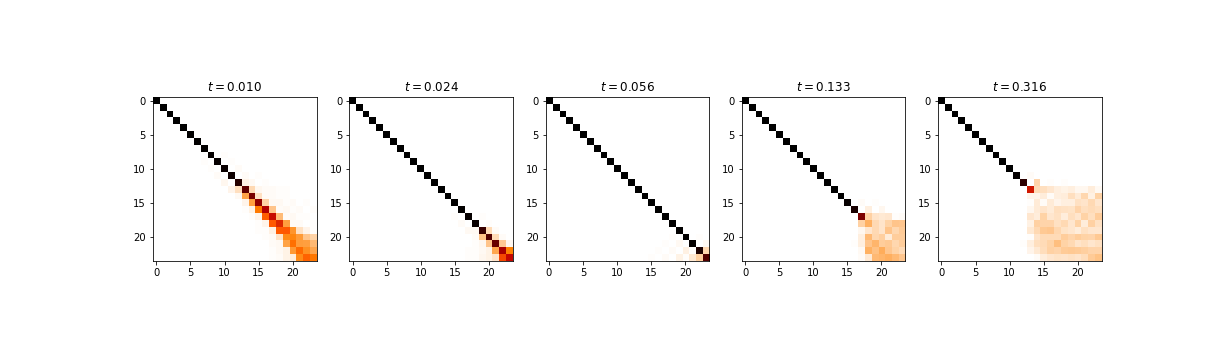
\includegraphics[width=\textwidth]{../codes/02.HeatKernelGraphLaplacian/HEALPix/06_figures/t_sensitivity}
	\caption{\label{fig:t_sensitivity_eigenspaces}Alignment of the eigenspaces of the HKGL with a fixed number of points $n$ corresponding to $N_{side}=8$}
\end{figure}
\begin{figure}
	\centering
	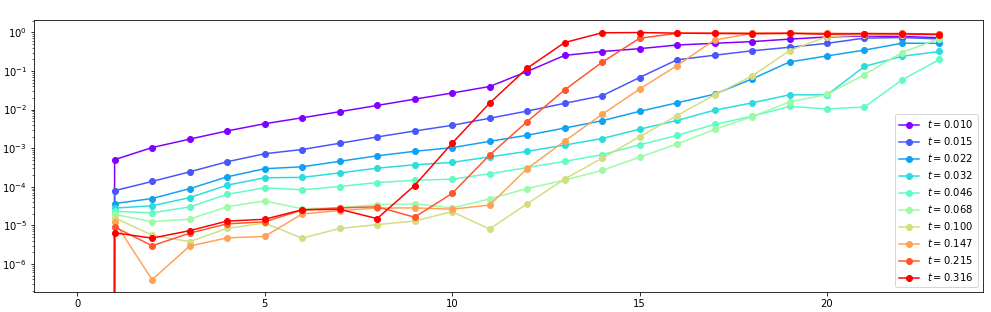
\includegraphics[width=\textwidth]{../codes/02.HeatKernelGraphLaplacian/HEALPix/06_figures/t_sensitivity_diagonal.png}
	\caption{\label{fig:t_sensitivity_diagonal}Whole trend}
\end{figure}%
\begin{figure}
	\centering
	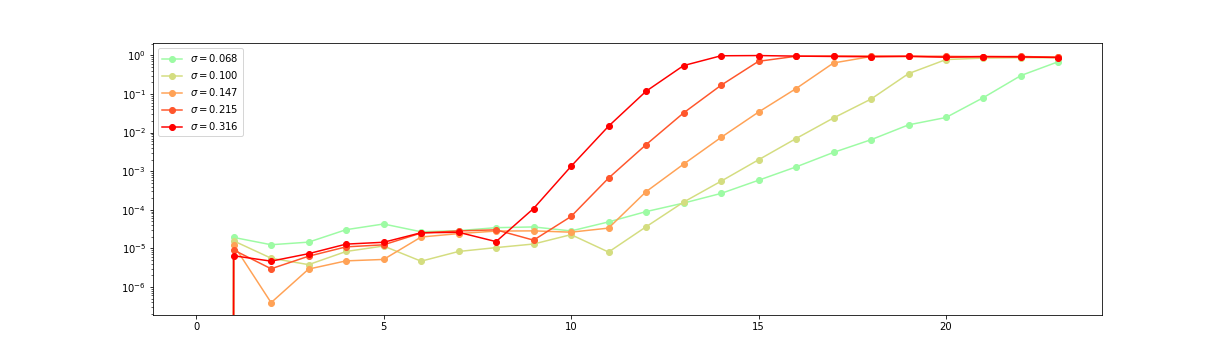
\includegraphics[width=\textwidth]{../codes/02.HeatKernelGraphLaplacian/HEALPix/06_figures/t_sensitivity_diagonal_2.png}
	\caption{\label{fig:t_sensitivity_diagonal_2}First trend: error stays low for low frequencies, and gets lower for high frequencies}
	\vspace{0.5cm}
\end{figure}
\begin{figure}
	\centering
	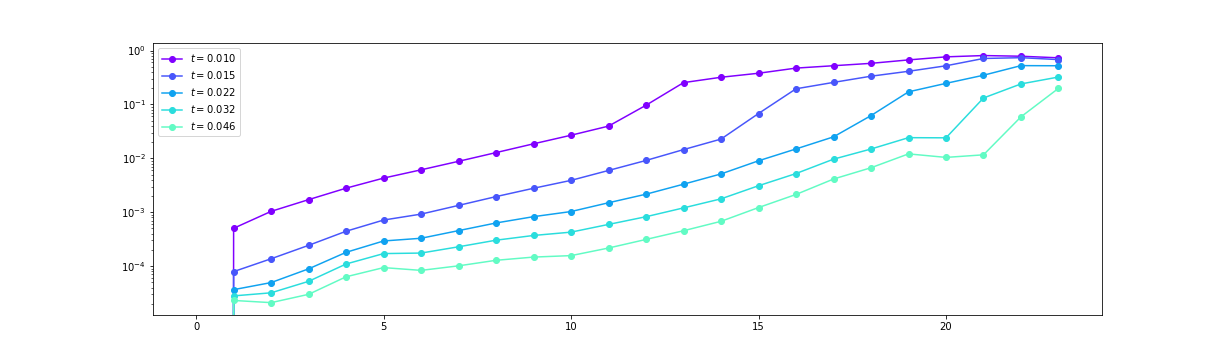
\includegraphics[width=\textwidth]{../codes/02.HeatKernelGraphLaplacian/HEALPix/06_figures/t_sensitivity_diagonal_1.png}
	\caption{\label{fig:t_sensitivity_diagonal_1}Second trend: error gets higher for both high and low frequencies}
\end{figure}%
\begin{figure}[h!]
	\centering
	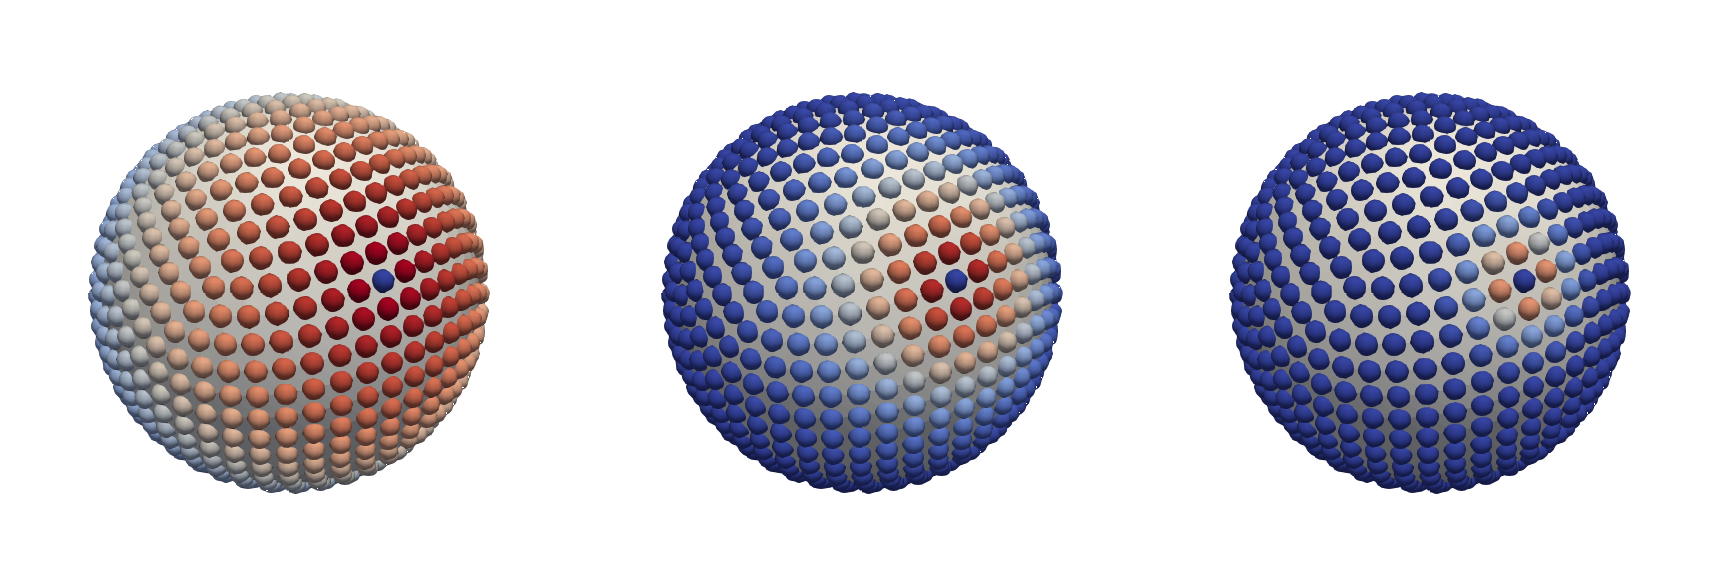
\includegraphics[width=\textwidth]{figs/chapter1/t.png}	
	\caption{\label{fig:weights}One row of the weight matrix for different values of the kernel width $t$ plotted on the HEALPix sampling with $N_{side}=8$. On the left, for a too large $t$, the HKGL can not capture high frequencies. On the right, for a too small $t$, the graph becomes almost completely disconnected. In the center a good value for $t$ makes the HKGL able to see the most frequencies.}
\end{figure}

Results are in figure \ref{fig:t_sensitivity_eigenspaces}, \ref{fig:t_sensitivity_diagonal}: Starting from $t=0.32$, the error in the high frequencies starts to get smaller, while the error in the low frequencies keeps staying low (Figure \ref{fig:t_sensitivity_diagonal_2}) up to $t=0.05$. For $t$ that gets smaller and smaller up to $t=0.01$, we get worse alignment both in high and low frequencies (Figure \ref{fig:t_sensitivity_diagonal_1}). This behavior can be explained with the same arguments used in the previous section: high values of the kernel width correspond to a very flat kernel (figure \ref{fig:weights}, left), and thus the graph loses the capacity of individuating high frequencies as discussed before. On the opposite side, low values of the kernel width correspond to a very peaked kernel, that causes all the weights to be close to zero and thus the graph becomes less and less connected loosing every capability of identifying different frequencies  (figure \ref{fig:weights}, right). 

\subsubsection{Putting it together: full graph, $n\to\infty$ and $t\to 0$}
A grid search has been used to find the following optimal kernel width for different values of $N_{side}$, always in the case of a full graph, where we maximized the number of graph eigenspaces with the alignment value in figure \ref{fig:optimal graph diagonal} bigger than $80\%$. The optimal values of the kernel width $t$ are shown in figure \ref{fig:t}, and the usual alignment plots in figures \ref{fig:optimal graph}, \ref{fig:optimal graph diagonal}. We can see in figure \ref{fig:t} that the heuristic way of \cite{DeepSphere} of setting the standard deviation $t$ produces results of the same order of magnitude of the optimal value. We recall that in DeepSphere $t$ is set to the average of the non zeros weight matrix entries, where the number of neighbors of each vertex is fixed between 7 and 8. It can be seen that the optimal values of $t$ are very close to a linear trend in the log-log plot, showing some kind of polynomial relationship with the parameter $N_{side}$ that could be used to extrapolate possible values of $t$ for higher $N_{side}$.
\begin{figure}[h]
	\centering
	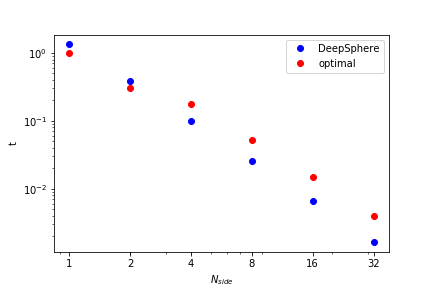
\includegraphics[width=0.7\textwidth]{../codes/02.HeatKernelGraphLaplacian/HEALPix/06_figures/kernelwidth.png}
\caption{\label{fig:t}Standard deviation of the Gaussian kernel  in a log-log plot. A straight line indicates a polynomial relation.}
\end{figure}
\begin{figure}[h]
	\centering
	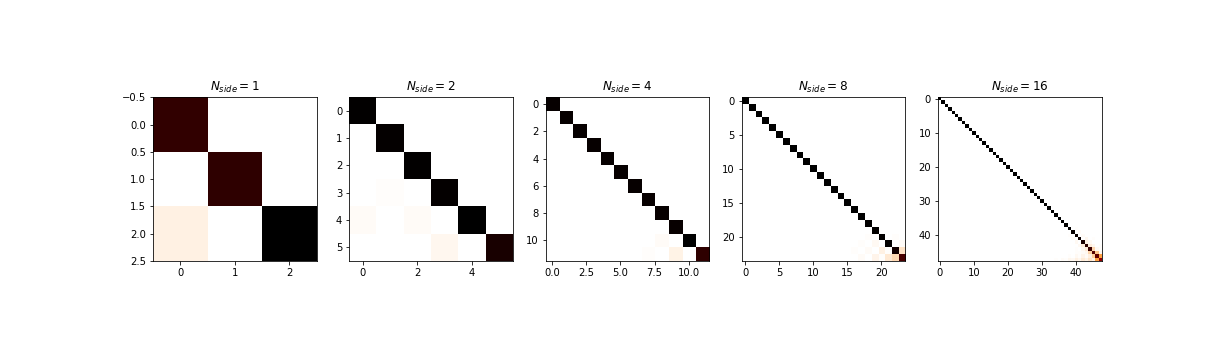
\includegraphics[width=\textwidth]{../codes/02.HeatKernelGraphLaplacian/HEALPix/06_figures/optimal_full.png}	
	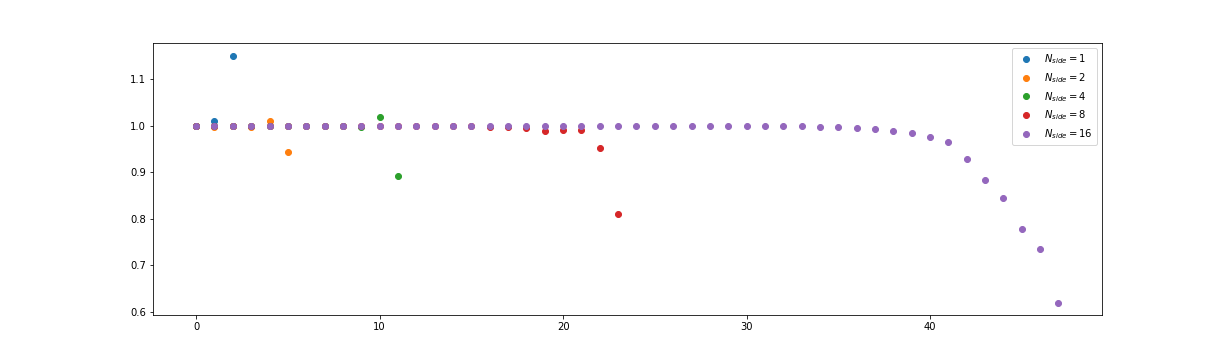
\includegraphics[width=\textwidth]{../codes/02.HeatKernelGraphLaplacian/HEALPix/06_figures/optimal_full_diagonal.png}
\caption{\label{fig:optimal graph}Alignment of eigenspaces for the optimal sequence $(t_n)$}
\end{figure}
In figure \ref{fig:optimal graph} we can appreciate that for a full graph, each time we double the parameter $N_{side}$, we approximately double the degree $\ell$ at which the graph eigenvectors are correctly aligned with the spherical harmonics.
\subsubsection{Reducing the number of neighbors}
For what it concerns how to make the graph sparse, the intuition is the following: remember that we want our graph Laplacian to approximate the operator $L^t$, that for sufficiently small $t$ approximates $\triangle$.
$$\frac{1}{n}\left(\sum_i e^{-\frac{||x_i-y||^2}{4t}}(f(y)-f(x_i)) \right) \quad \approxeq \quad \int_\mathcal M e^{-\frac{||x-y||^2}{4t}}\left(f(y)-f(x)\right)d\mu(x) $$

So far we showed how to do so optimally with a full graph; however, a full graph comes at the cost of leading to a matrix $\mathbf L_n^t$ that is full and thus to a graph filtering of the order of $\mathcal O(n^2)$. We want now to make the graph sparse such that the number of non-zero entries of the Laplacian is $\mathcal O (n)$, making the graph filtering linear in the number of pixels. For this reason Perraudin et al. \cite{DeepSphere} construct a nearest neighbor graph constraining the number of neighbors for each vertex to be less than 8. However, as we saw at the beginning of this section this leads to a poor alignment of the graph eigenvectors with the spherical harmonics and thus to a not so optimal rotation equivariance. Here we propose a different approach, based on the following intuition: making the graph sparse means deciding which weights $W_{i,j}=\exp{-\frac{||x_i-x_j||^2}{4t}}$ to set to $0$. For this approximation to be accurate we want to set to 0 only those weights that are small enough: let's define a new \textit{epsilon graph} $W'$ by fixing a threshold $\epsilon$ on $w_{i,j}=e^{-\frac{||x_i-x_j||^2}{4t}}$ such that

$$W'_{i,j} = \begin{cases}
e^{-\frac{||x_i-x_j||^2}{4t}}\quad& \text{if } e^{-\frac{||x_i-x_j||^2}{4t}} \geq \epsilon\\
0 \quad & \text{if } e^{-\frac{||x_i-x_j||^2}{4t}} < \epsilon
\end{cases}$$

By setting $\epsilon = 0.01$ - or equivalently, thresholding the weights at $\norm{x_i-x_j}\approx 3\sigma$ where $\sigma=\sqrt{2t}$ is the standard deviation of the kernel - in figure \ref{fig:optimal_thresholded} we can see the usual alignment plots for the graph $W'$:

\begin{table}[h]
	\centering
	\begin{tabular}{ c|c} 
		$N_{side}$ & Number of neighbors \\ 
		1 & 11 \\ 
		2 & 16 \\ 
		4 & 37 \\ 
		8 & 43 \\ 
		16 & 52 \\ 
	\end{tabular}
\caption{\label{table:NN}}
\end{table}

\begin{figure}[h]
	\centering
	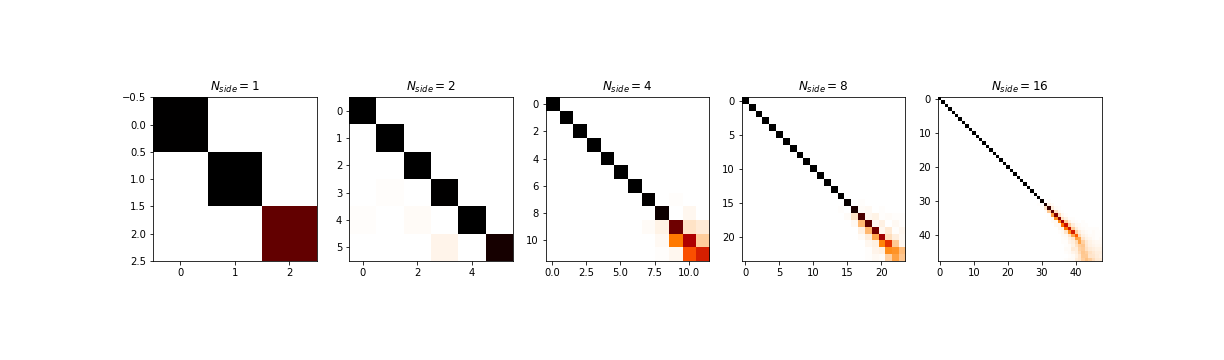
\includegraphics[width=\textwidth]{../codes/02.HeatKernelGraphLaplacian/HEALPix/06_figures/optimal_thresholded.png}	
	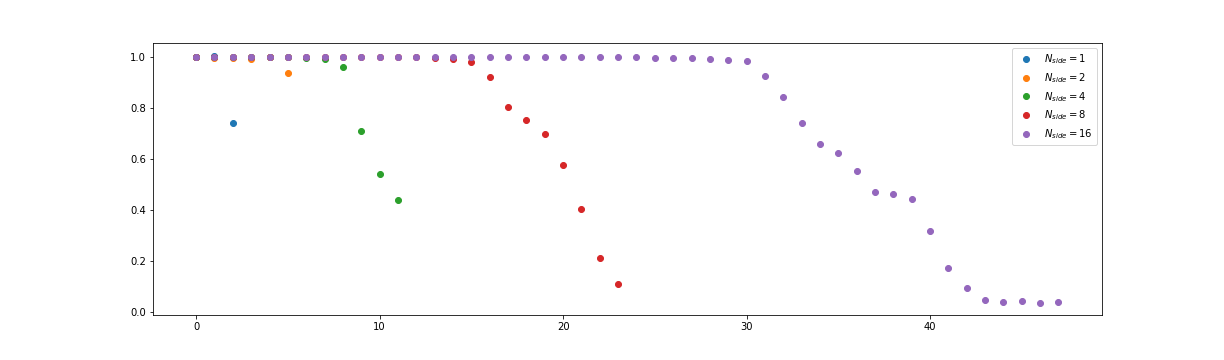
\includegraphics[width=\textwidth]{../codes/02.HeatKernelGraphLaplacian/HEALPix/06_figures/optimal_thresholded_diagonal.png}
	\caption{\label{fig:optimal_thresholded}Optimal construction \textbf{thresholded at $k=0.01$}}
\end{figure}

We see that we need to increase the number of neighbors as $N_{side}$ gets bigger. Again, the intuition is the following: to have spectral convergence (a strong type of convergence) we need more and more global information and more precise. By fitting the relationship
$$
\text{Number of neighbors} = (N_{side})^\alpha
$$
to the data in table \ref{table:NN} we obtain that $\alpha$ should be close to $1/2$, meaning that the complexity of DeepSphere optimal could be approximated by
$$
\mathcal O(|E|) = \mathcal O(n\sqrt{N_{side}})  = \mathcal{O}(n^{5/4}).
$$
where $n$ is the number of vertices of the graph. This complexity is a little worse that the linear complexity of DeepSphere, but in practice the number of neighbors grows very slowly with the number of pixels, making graph convolutions still computationally efficient (see section \ref{sec:Chapter2:Experimental validation}, table \ref{table:results}). 

To conclude this subsection, we show in figure \ref{fig:Old spectrum}, \ref{fig:New spectrum} we show a confront between the alignment of the graph Laplacian eigenvectors and the spectra of the DeepSphere graph $W$, the starting point of this work, and  of the proposed graph $W'$. It can appreciated how the alignment plots show a much better behavior of the graph Laplacian eigenvectors, and how the eigenvalues show now the correct multiplicity. This was obtained through a careful selection of the kernel width $t$ and of the number of neighbors in accord with the theory developed in the previous section. \\
\begin{minipage}{.5\textwidth}
	\centering
	\vspace{0.4cm}
	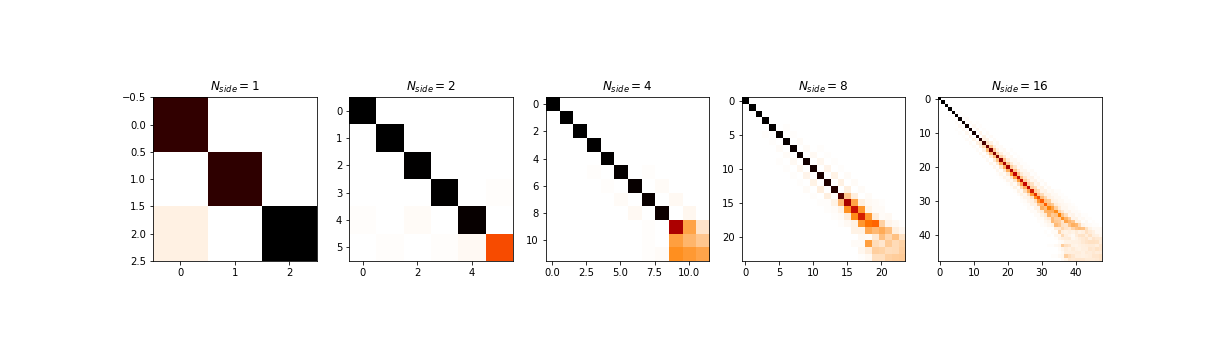
\includegraphics[width=0.95\linewidth]{../codes/02.HeatKernelGraphLaplacian/HEALPix/06_figures/deepsphere_original.png}
	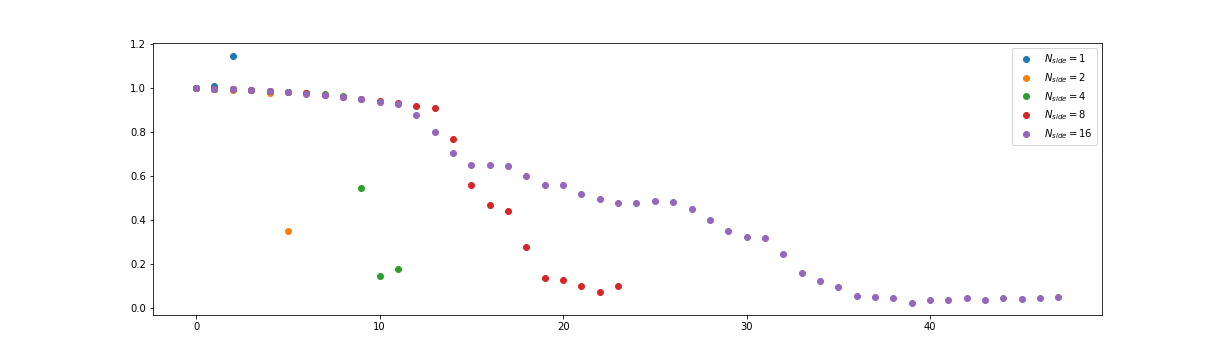
\includegraphics[width=0.95\linewidth]{../codes/02.HeatKernelGraphLaplacian/HEALPix/06_figures/deepsphere_original_diagonal.png}
	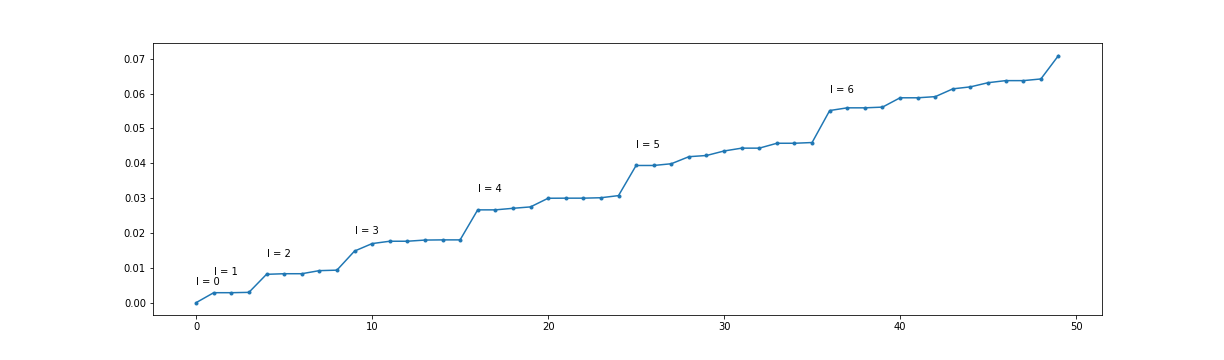
\includegraphics[width=0.95\linewidth]{../codes/02.HeatKernelGraphLaplacian/HEALPix/05_figs/old_results3.png}
	\captionof{figure}{\label{fig:Old spectrum}Alignment of the graph Laplacian eigenvectors of the DeepSphere graph $W$, the starting point of this work, and its spectrum.}
\end{minipage}%
\begin{minipage}{.5\textwidth}
	\centering
	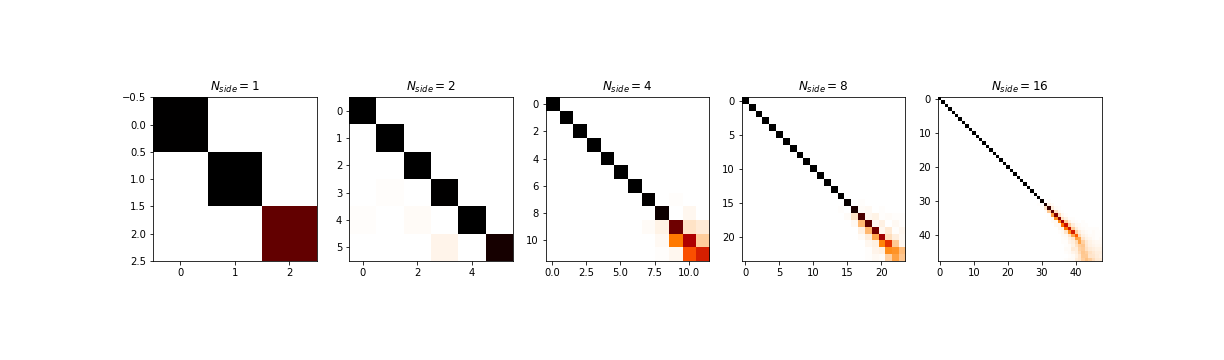
\includegraphics[width=0.95\linewidth]{../codes/02.HeatKernelGraphLaplacian/HEALPix/06_figures/optimal_thresholded.png}
	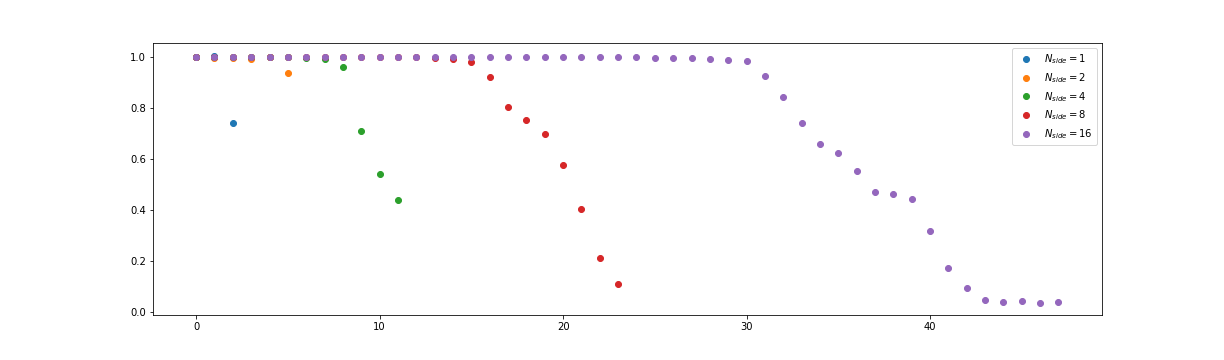
\includegraphics[width=0.95\linewidth]{../codes/02.HeatKernelGraphLaplacian/HEALPix/06_figures/optimal_thresholded_diagonal.png}
	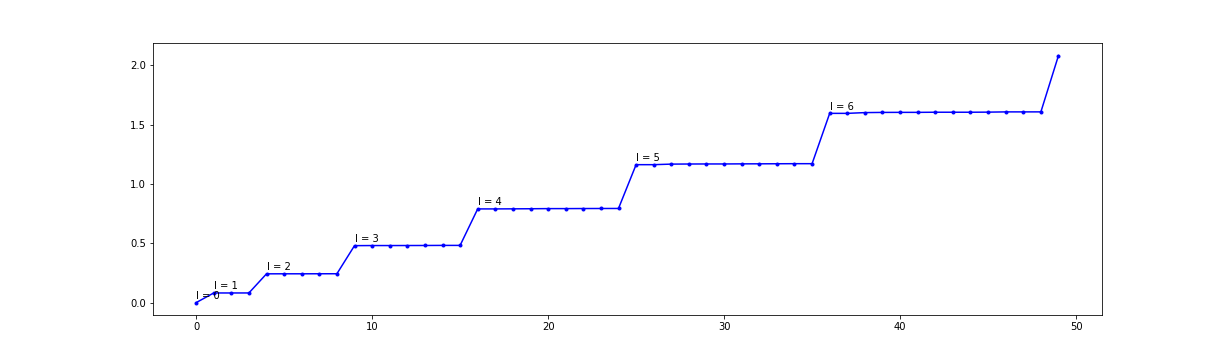
\includegraphics[width=0.95\linewidth]{../codes/02.HeatKernelGraphLaplacian/HEALPix/06_figures/optimal_thresholded_eigenvalues.png}
	\captionof{figure}{\label{fig:New spectrum}Alignment of the graph Laplacian eigenvectors of the proposed graph $W'$ and its spectrum.}
\end{minipage}
\subsubsection{Equivariance error}
So far we used the alignment of the eigenvectors with the spherical harmonics as a proxy of the quantity we are really interested in, the mean equivariance error $\overline E_G$, because it gave us more valuable interpretations about what was happening thus it was easier to tune and find the optimal parameters. Now we want to have the confirmation that the proposed graph $G'$ led to a smaller mean equivariance error than the one of the original graph $G$ of DeepSphere.
In figures \ref{fig:DeepSphere equivariance error} and we plot the mean equivariance error 
$$\overline E = \mathbb E_{f, g}\ E(f, g)
$$ of the diffusion filter $K = \exp(-\Lambda)$ for both graphs $G, G'$ by spherical harmonic degree $\ell$ for a fixed $N_{side}=8$. This was obtained as the empirical average over a uniform sample of rotations $g\in SO(3)$ and a uniform sample of functions $f\in V_\ell = \text{span}\{Y_\ell^m, |m|\leq \ell\}$. We recall that for HEALPix there's no sampling theorem that guarantees the existence of an exact reconstruction operator $T^{-1}$, so to calculate this quantity we had to rotate the sampled signal in the discrete domain, introducing important interpolation errors. We can see that DeepSphere has a mean equivariance error that is almost 30\% already for the low frequencies, and decreases slowly for higher ones but always stays above 10\%. The graph $G'$ has a much better behavior: the error stays low for the smaller frequencies, rising up for the higher ones and always remaining confined under 5\%. To compare it we reported also the results for the full HKGL, where we can appreciate a behavior similar to $G'$ but with an error always smaller than 2\%.

\begin{figure}[h]
	\centering
	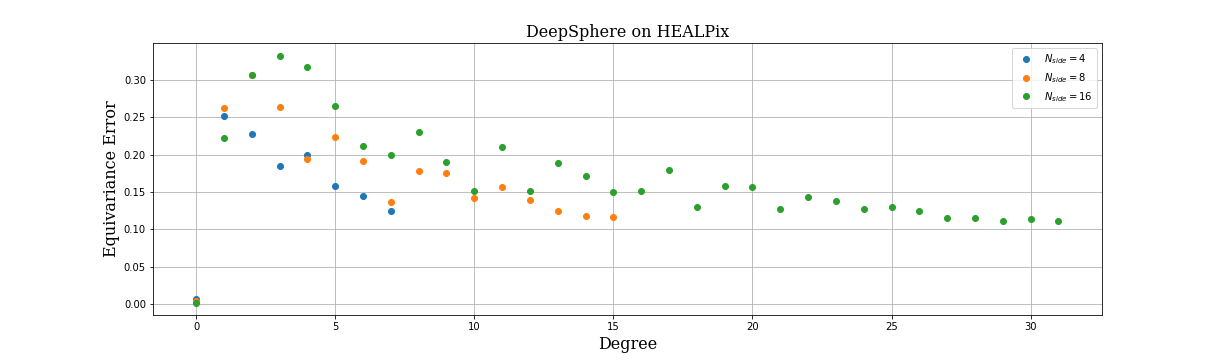
\includegraphics[width=\textwidth]{../codes/06.Equivariance_error/DeepSphereonHEALPix.png}	
	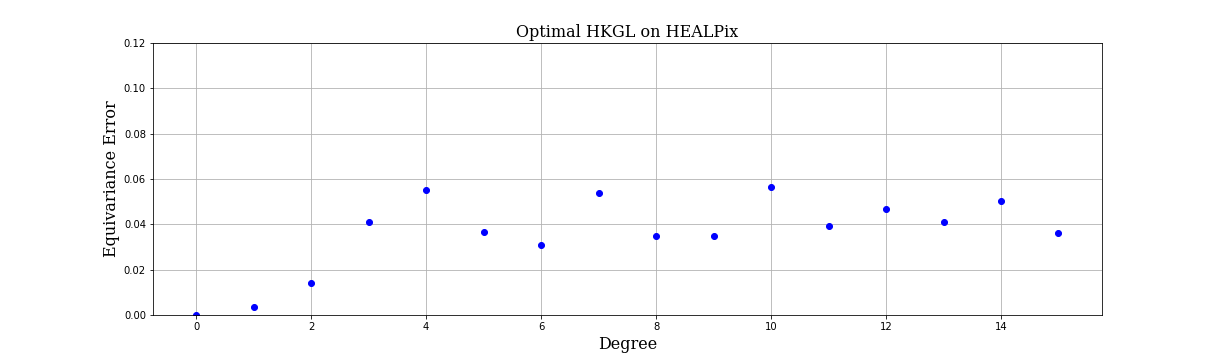
\includegraphics[width=\textwidth]{../codes/06.Equivariance_error/OptimalHKGLonHEALPix.png}	
		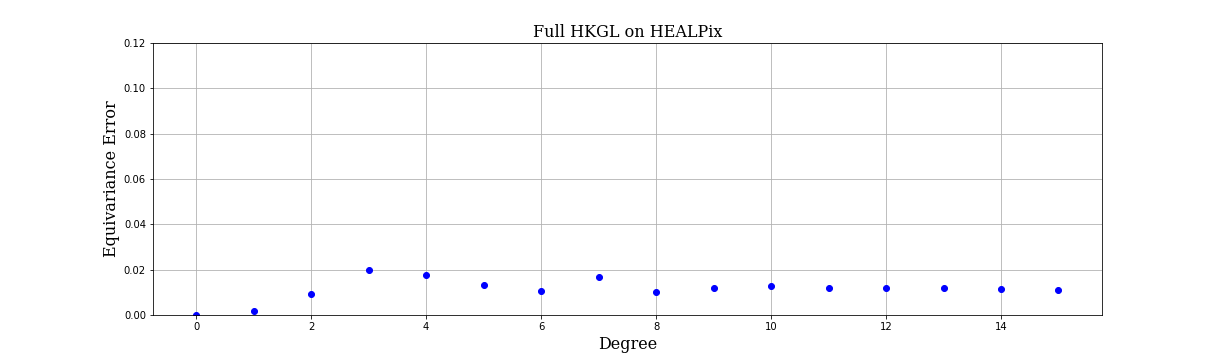
\includegraphics[width=\textwidth]{../codes/06.Equivariance_error/FullHKGLonHEALPix.png}	
	\caption{\label{fig:DeepSphere equivariance error}Mean equivariance error of the diffusion filter $\exp(-\Lambda)$ for $G$, $G'$ and the full HKGL, by spherical harmonic degree. Notice the difference in the scale of the y axis for DeepSphere, that reaches errors up to 30\%.}
\end{figure}

\begin{figure}[h!]
	\centering
	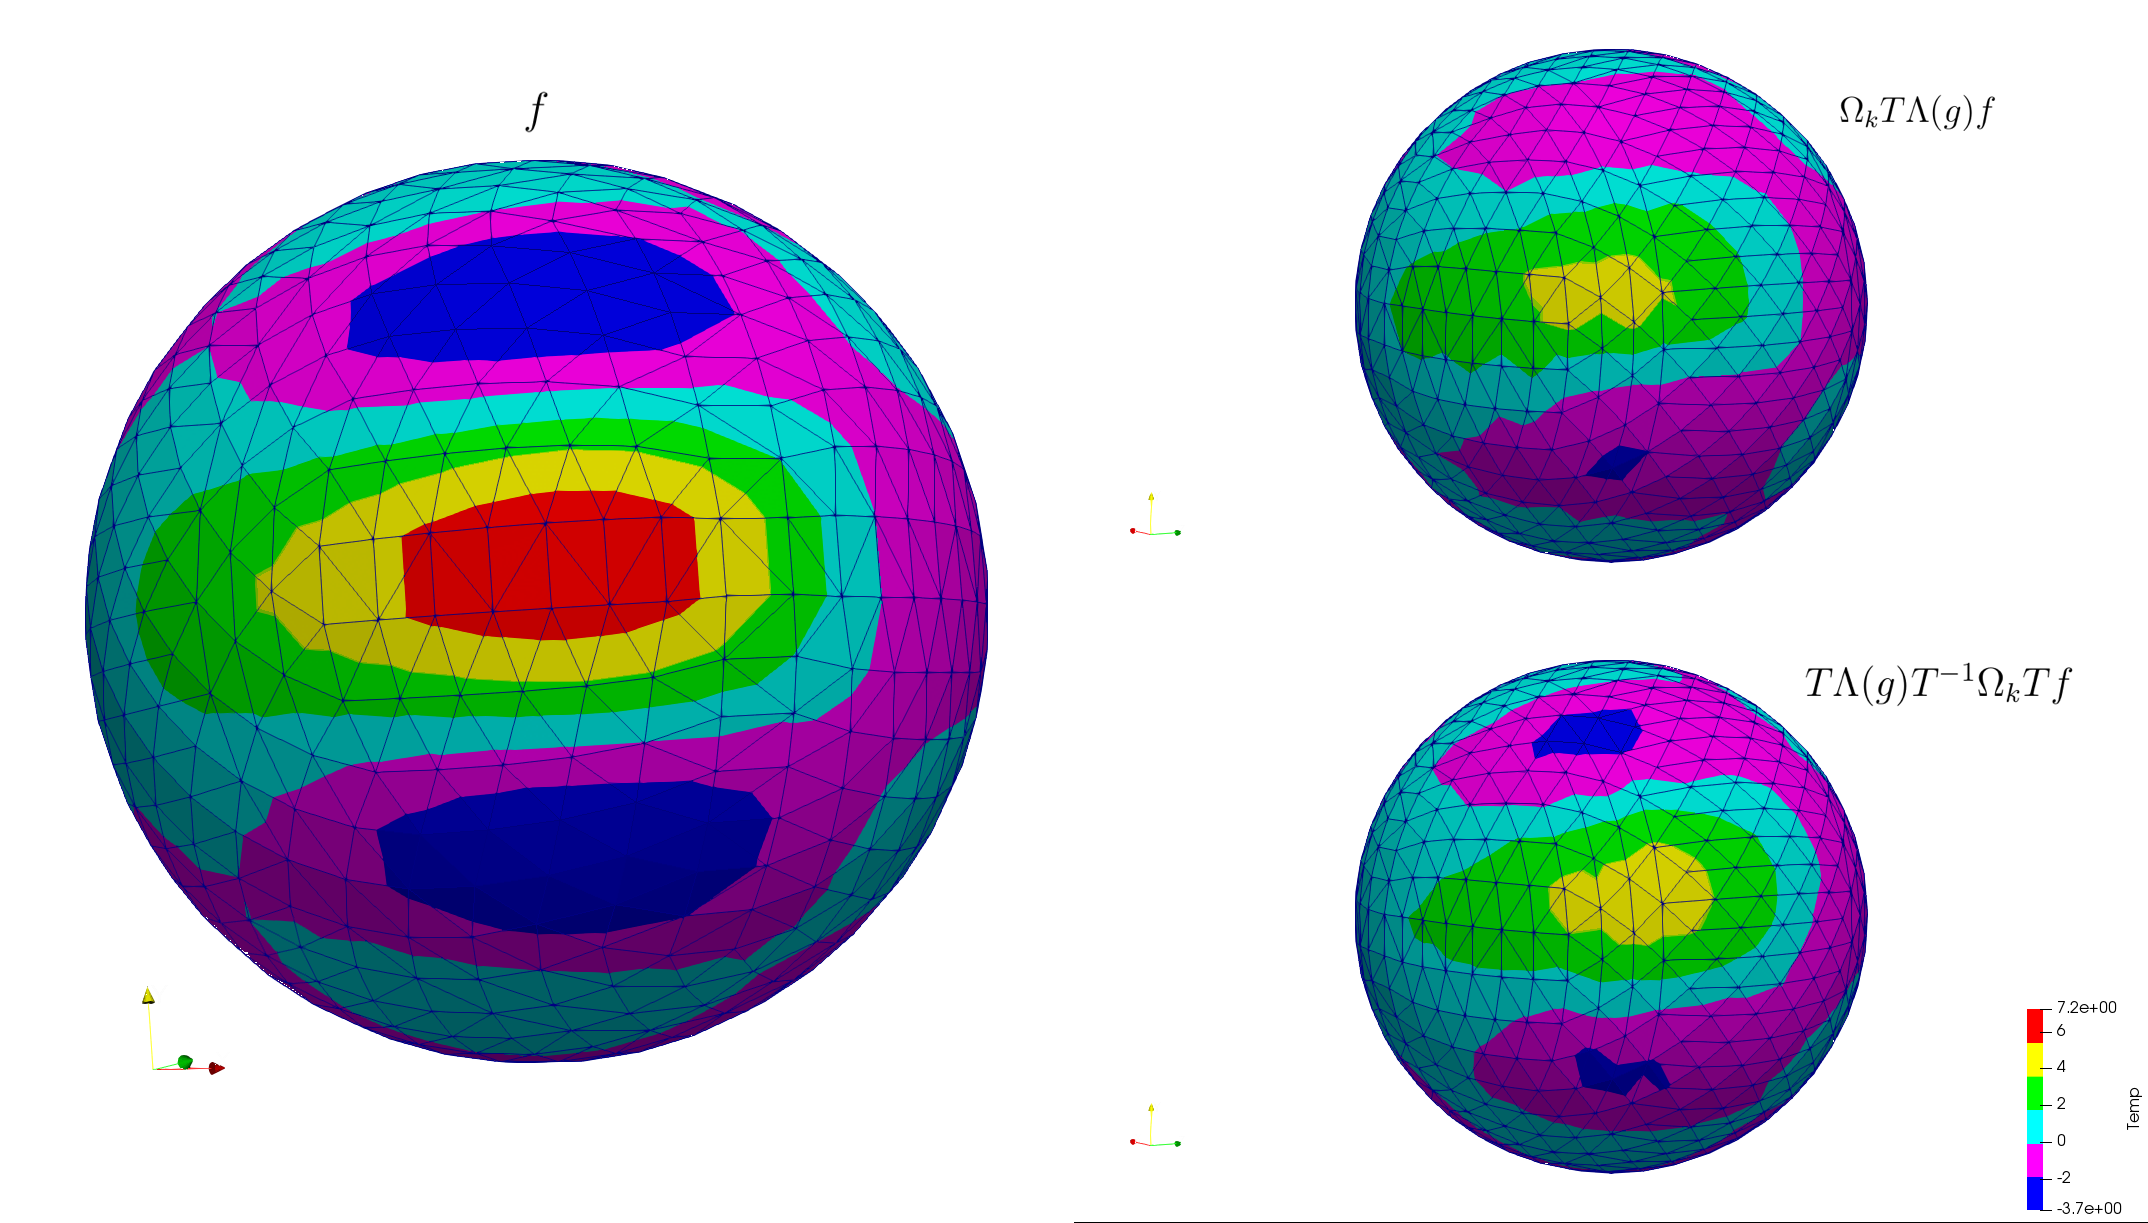
\includegraphics[width=\textwidth]{../codes/06.Equivariance_error/img_example_DeepSphere/DS.png}	
	\caption{\label{fig:DeepSphere equivariance error in practice}DeepSphere V1 equivariance error. On the left, a signal $f$. Top right, $f$ was first rotated and then filtered through a diffusion filter $k(\lambda) = \exp (-\lambda)$. Bottom right, $f$ was first filtered and then rotated. The difference in the two outcomes is evident.}
\end{figure}


\begin{figure}[h!]
	\centering
	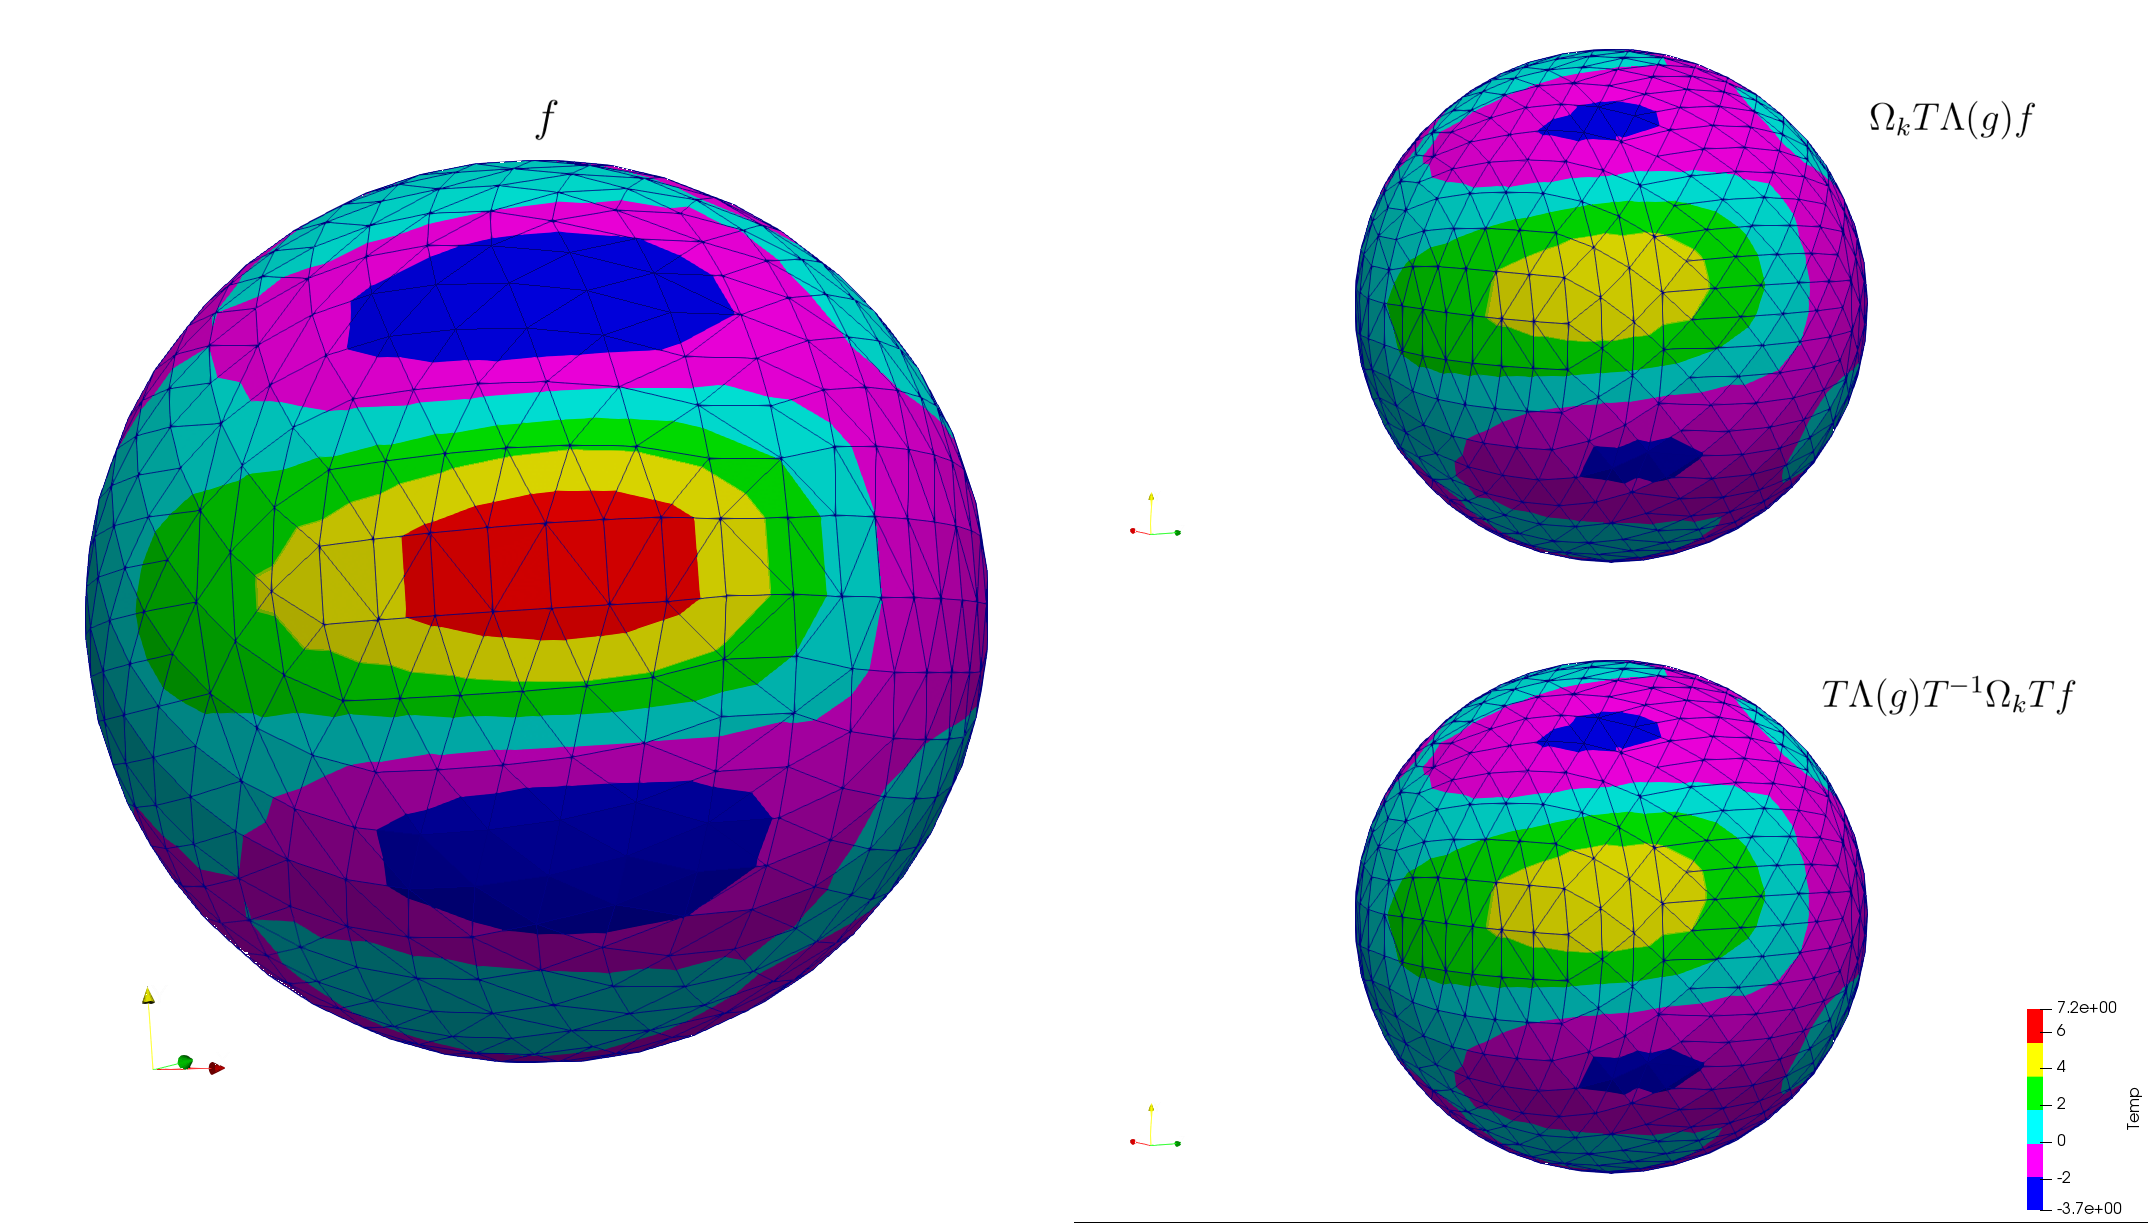
\includegraphics[width=\textwidth]{../codes/06.Equivariance_error/img_example_thresholdedHKGL/thresholdedHKGL.png}	
	\caption{\label{fig:Optimal equivariance error in practice}DeepSphere V2 equivariance error. On the left, a signal $f$. Top right, $f$ was first rotated and then filtered through a diffusion filter $k(\lambda) = \exp (-\lambda)$. Bottom right, $f$ was first filtered and then rotated. No difference in the two outcomes is visible to the human eye.}
\end{figure}

In figure \ref{fig:DeepSphere equivariance error in practice} we see the visualization of the equivariance error of DeepSphere: on the left, the original sampled signal $Tf$. Top right, the rotated and filtered signal $\Omega_k T \Lambda(g) f$. Bottom right, the filtered and rotated signal $T \Lambda(g) T^{-1} \Omega_k T f $. The difference between them can be appreciated. In figure \ref{fig:Optimal equivariance error in practice} we see the visualization of the equivariance error of the optimal graph $G'$: on the left, the same original sampled signal $Tf$. Top right, the rotated and filtered signal $\Omega_k T \Lambda(g) f$. Bottom right, the filtered and rotated signal $T \Lambda(g) T^{-1} \Omega_k T f $. No difference between them can be appreciated at a visual analysis.
To conclude, we report in table \ref{tab:final results} as final metric for the evaluation of rotation equivariance of the two graphs $G$, $G'$ the mean equivariance error for a different values of $N_{side}$ that we computed by sampling random coefficients $\theta_\ell^m \in(0,1)$ of linear combinations of all the spherical harmonics up to degree $\ell=16$
$$f(x) = \sum_{\ell\leq 16,\ |m|\leq\ell}\theta_\ell^m Y_\ell^m(x)
$$
and by averaging on random rotations $g\in SO(3)$. Our graph shows lower errors as $N_{side}$ grows, and a much lower error than DeepSphere.

\begin{table}
		\centering
\begin{tabular}{c|ccc}
	Mean equivariance error $\overline{E}$& $N_{side}=4$& $N_{side}=8$&$N_{side}=16$ \\\hline
	DeepSphere graph $G$ & 12.37\% & 12.03\% & 12.23\% \\
	Optimal graph $G'$ & 4.57\% & 3.98 \% & 1.54\%
\end{tabular}
\caption{\label{tab:final results}}
\end{table}

